\documentclass[a4paper,fleqn]{cas-dc}
\usepackage{cleveref}
\usepackage{placeins}
\usepackage{afterpage}
\usepackage{rotating}
\usepackage{adjustbox}
\usepackage{array}
\usepackage{xcolor}
\usepackage{subcaption}

\newcolumntype{F}{@{\extracolsep{\fill}}>{\global\let\currentrowstyle\relax}l}  % apply row style to column, similar to L
\newcolumntype{H}{@{\extracolsep{\fill}}>{\currentrowstyle}>{\bfseries}c}  % adds bold face to column, similar to C
\newcolumntype{K}{@{\extracolsep{\fill}}>{\currentrowstyle}c}  % forward F style to next columns
\newcolumntype{B}{@{\extracolsep{\fill}}>{\currentrowstyle}>{\color{blue}}c}  % apply blue color to column, similar to C

\newcolumntype{f}{@{\extracolsep{\fill}}>{\global\let\currentrowstyle\relax}>{\color{blue}}l}  % apply row style to column, similar to L
\newcolumntype{o}{@{\extracolsep{\fill}}>{\currentrowstyle}>{\color{blue}}l}  % apply blue color to column, similar to B

\newcommand{\rowstyle}[1]{\gdef\currentrowstyle{#1}#1\ignorespaces}  % apply row style
\newcommand{\bfrow}{\rowstyle{\bfseries}}  % apply bold face to row
\newcommand{\bluerow}{\rowstyle{\color{blue}}}  % apply blue color to row
\newcommand{\responsemod}{\color{blue}}
\newcommand{\responsemodsm}[1]{\textcolor{blue}{#1}}
\newcommand{\captionb}[1]{\caption{\responsemodsm{#1}}}
\usepackage[authoryear]{natbib}

\def\tsc#1{\csdef{#1}{\textsc{\lowercase{#1}}\xspace}}
\tsc{WGM}
\tsc{QE}

\renewcommand{\dblfloatpagefraction}{0.4}

\begin{document}
\let\WriteBookmarks\relax
\def\floatpagepagefraction{1}
\def\textpagefraction{.001}

\shorttitle{Weightage-based Supervised Learning System.}

\shortauthors{Ketkar Y., Gawade S.}

\title [mode = title]{Detection of Arrhythmia Using Weightage-based Supervised Learning System for COVID-19.}

\let\printorcid\relax

\author[1]{Yashodhan Ketkar}

\ead{ketkaryapr19me@student.mes.ac.in}

\affiliation[1]{organization={Department of Information Technology Engineering, Pillai College of Engineering},
    city={Panvel},
    postcode={410206},
    state={Maharashtra},
    country={India}}

\author[2]{Sushopti Gawade}

\ead{sgawade@mes.ac.in}

\affiliation[2]{organization={Department of Computer Engineering, Pillai College of Engineering},
    city={Panvel},
    postcode={410206},
    state={Maharashtra},
    country={India}}

\begin{abstract}
    COVID-19 disease has became a global pandemic in the last few years. This disease was highly contagious, and it quickly spread throughout several countries. Its infection can lead to severe implications for its victims, including cardiovascular issues. This complication develops in some people with a history of cardiovascular illness, whereas it emerges in others after COVID-19 infection. Cardiovascular problems are the primary cause of mortality in COVID-19 patients and are used to predict disease prognosis. Identifying arrhythmia from abnormalities in patient ECG signals is one approach to the detection of cardiovascular disorders. This is a laborious and time-consuming procedure that can be automated. The proposed method selects the most suitable model for this task. The selection is made through the weightage generated from the user's requirements. The proposed method uses supervised learning to identify abnormalities in ECG waves. The models provided by the selection system during tests were able to meet user requirements. The models achieved up to 97\% accuracy and 97\% precision in predictive tasks.
\end{abstract}

\begin{keywords}
    Arrhythmia Detection \sep
    Automated Model Generation \sep
    Automated Model Training \sep
    Machine Learning In Healthcare \sep
    Supervised Learning Algorithms \sep
    Weightage based Model Selection \sep
\end{keywords}

\tolerance 9999
\maketitle

\begin{table}
    \begin{tabular*}{\tblwidth}{@{}ll@{}}
        \multicolumn{2}{l}{\bfseries Table of Acronyms} \\
        \toprule
        \textbf{ACRONYMS} & \textbf{DEFINITION} \\
        \midrule
        COVID-19 & Coronavirus Disease 2019 \\
        ECG & Electrocardiogram \\
        AutoML & Automated Machine Learning \\
        LDA & Linear Discriminant Analysis \\
        ML & Machine Learning Learnign \\
        SVM & Support Vector Machine \\
        KNN & K-Nearest Neighbors \\
        DT & Decision Tree \\
        RPA & Robotic Process Automation \\
        LSTM & Long Short-term Memory \\
        MLP & Multilayer Perceptron \\
        HIPAA & Health Insurance Portability and Accountability \\
        & Act \\
        TP & True Positive \\
        TN & True Negative \\
        FP & False Positive \\
        FN & False Negative \\
        ROC & Receiver Operating Characteristic \\
        MIT-BIH & Massachusetts Institute of Technology-Beth \\
        & Israel Hospital.\\
        %
        RF & Random Forest \\
        \bottomrule
    \end{tabular*}
\end{table}

\FloatBarrier
\section{Introduction} \label{sec:introduction}

COVID-19 has been widespread in recent years. It targets the human respiratory system, causing severe respiratory issues. Depending on a person's condition and the prevalence of comorbidities, this disease can be fatal. COVID-19 disease frequently causes cardiovascular comorbidities. Cardiovascular comorbidities are also problematic to diagnose in the absence of suitable equipment. Checking for arrhythmia in patients is one approach to detection. Arrhythmia is the irregular beating of the heart. Arrhythmia is detected by examining ECG signals. Because COVID-19 has put a strain on the medical personnel, detection takes longer than usual. Increased Internet connectivity has led to the use of machine learning and artificial intelligence (AI) for service in a variety of sectors. This increases research in the field of machine learning and has an impact on machine learning in a variety of domains. One of them is the medical and healthcare industries. Machine learning is used to detect and categorize viruses and other microorganisms in patients. In medical applications, machine learning algorithms have already been shown to be quite useful.

The machine learning system may be used to scan these ECG signals and detect them. These signs may be detected considerably faster and more efficiently using supervised learning techniques. In such exact classification problems, supervised algorithms have previously been demonstrated to be quicker than unsupervised techniques. Once taught, this algorithm may also be utilized to make future predictions.

There are several supervised algorithms available, allowing us to select the best method for our purposes. This phase can be automated in the case of the general population. A few methods may be pre-programmed into the system, and the computer can then train and pick the best model for the supplied dataset. This will free up medical personnel to focus on patient care and problem-solving.

\FloatBarrier
\section{Literature Review} \label{sec:literature_review}

\cite*{02_rp} suggest that arrhythmia is one of the most common symptoms in patients with COVID19. Arrhythmia was found in 7\% of all Wuhan COVID-19 cases and 14.8\% of patients with poor outcomes. \cite*{18_rp} state that 17\% of patients hospitalized in China were diagnosed with arrhythmia. \citeauthor{18_rp} conducted a review of 10 eligible studies (5,193 patients) for analysis and found that atrial arrhythmia was present in 9.2\% of cases. A review by \cite*{15_rp} of 17 studies with 5,815 patients showed that arrhythmia was detected in 9.3\% of COVID-19 cases. \cite*{25_rp} suggest that only 8\% of patients with arrhythmia had prior cardiovascular conditions. \citeauthor{25_rp} also mentioned that 56\% of patients showed symptoms after the COVID-19 infection.

\cite*{24_rp} used an ensemble classifier to detect the anomalies in the ECG signal. This approach, which combines multiple classifiers for prediction, has proven effective because the accuracy of the ensemble classifier is significantly higher than that of a single classifier. A few authors used this approach to improve the prediction accuracy of supervised learning models. \cite*{10_rp} used the maximal overlap wavelet packet transform ensemble with a neural network and achieved satisfactory results. \cite*{20_rp} used the ensemble approach to predict the results of the students. \citeauthor{20_rp} state the model was able to predict the correct results even with a small amount of training data. \cite*{16_rp} compared the FLINK-based iForest ensembled algorithms against the sklearn-iForset and other algorithms. \citeauthor{16_rp} concluded that the Flink-iForest algorithm showed better performance than off-the-shelf algorithms. \cite*{11_rp} used the AutoML algorithm and tools on data streams. \citeauthor{11_rp} concluded that the default classifiers can be used with AutoML tools for accurate prediction. With AutoML tools, prediction systems can be automated.

\cite*{ref_paper_m1} used machine learning for the prediction of end-of-semester results. \cite*{ref_paper_m1} used SVM, KNN, and DT models. \cite*{ref_paper_m1} concluded that the machine learning system performed satisfactorily, with SVM achieving up to 78\% accuracy.

\cite*{23_rp} extracted appropriate features for the detection of epileptic seizures. \citeauthor{23_rp} preprocessed data and used ML algorithms on the data. \citeauthor{23_rp} concluded that the supervised learning models showed more effectiveness than the unsupervised learning models. \cite*{12_rp} used a commercial classifier for the detection of arrhythmia. \citeauthor{12_rp} used ECG signals from patients and applied a custom SVM classifier. \citeauthor{12_rp} concluded that the algorithm was a successful and efficient detector of arrhythmia.

\cite*{ref_paper_m2} used supervised learning algorithms for the early detection of heart disease and diabetes disease. \cite*{ref_paper_m2} concluded that the model performed satisfactorily.

\cite*{09_rp} used neural networks to process raw ECG signals and make predictions. While \cite*{22_rp} used small neural networks for efficient recognition processes, both studies concluded that artificial neural networks are extremely efficient and accurate in the prediction of anomalies.

\cite*{06_rp} showed that the LDA classifier can outperform the SVM classifier in low-performance environments and lightweight systems. The self-learning algorithm makes the system more dynamic and adaptable to incoming signals. \cite*{14_rp} used adaptive fuzzy algorithms to classify ECG signals. \citeauthor{14_rp} stated that the algorithm showed satisfactory results, but it requires prior classification patterns results. \cite*{ref_paper_self_rpa} suggest that the RPA system can be used in these systems for easier integration of machine learning with dynamic data. \cite*{21_rp} used ECG signals of COVID-19 patients for patient monitoring. \citeauthor{21_rp} used LSTM, SVM, and MLP algorithms to monitor data. \citeauthor{21_rp} suggest that machine learning with robotics can provide better results.

\cite*{07_rp} used a multi perceptron neural network for stroke predictions. The neural network showed high accuracy. \citeauthor{07_rp} were able to achieve up to 78\% accuracy. \citeauthor{07_rp} suggest that the model can produce better results with a larger training dataset. \cite*{05_rp} used artificial intelligence to detect heart disease. \citeauthor{05_rp} concluded that the algorithms achieved up to 83\% accuracy. \citeauthor{05_rp} also concluded that the system was able to comply with the HIPAA regulations.

\cite*{ref_paper_m3} used machine learning algorithms to predict crop growth rates. \citeauthor{ref_paper_m3} were able to get good insights into the field. \citeauthor{ref_paper_m3} concluded that the use of machine learning will result in minimizing complexity and increasing yield in farming.

\cite*{01_rp} used a two-year dataset collected by Glumo Lake and used their expertise to train and select models. A mixed approach of data-driven and knowledge-driven modeling is used for the success of the application. \cite*{13_rp} used loo rate and stop criteria for model selection. \citeauthor{13_rp} investigated eight different issues and found that a larger loo rate was more desirable. \citeauthor{13_rp} also suggested that modeling difficulties can only be found by careful numerical calculations.

\cite*{17_rp} used a novel kernel to get the dataset description. \citeauthor{17_rp} concluded that this approach led to the discovery of invisible models. \citeauthor{17_rp} also state that this approach reduces the amount of human interaction. \cite*{04_rp} created a new model using the glmulti package. These models are unique and flexible. The model is automatically optimized to provide a multi-model interface. This approach allows you to quickly explore a large set of models for selection purposes. \cite*{08_rp} optimized parameters with a genetic algorithm. \citeauthor{08_rp} successfully used a genetic algorithm to reduce uncertainty in the prediction results. These methods can be used for the automated model selection system.

\FloatBarrier
\section{Methodology} \label{sec:methodology}

\subsection{Mathematical Model}\label{subsec:mathematical_model}

\Cref{fig:model_selection_approach} shows the approach to the selection of a suitable model. The system can handle an infinite number of models. For each model, six performance parameters are used. These performance metrics are accuracy P$_1$, F1 score P$_2$, precision P$_3$, recall P$_4$, area under the ROC P$_5$, and prediction time P$_6$. From these, the first five parameters are grouped and given a weightage range between 0.2 and 1.0, whereas prediction time is given a weightage range between 0.25 to 0.75. \Cref{eq:v_score} shows the mathematical formula used to calculate the Vscore of the models.

For models M$_1$, M$_2$,..., M$_n$, the Vscores V$_1$, V$_2$,..., V$_n$ are obtained. These obtained Vscores are compared with each other. The model with the highest Vscore is selected as the most-suited model.

\begin{equation}\label{eq:v_score}
    V_{score} = \left(\sum_{x=1}^{5} w_xP_x\right) - w_6^2P6
\end{equation}

\begin{itemize}
    \item[where,]
    \item[$V_{score}$] Vscore of the model
    \item[$w_x$] The weightage generated by the system for the $x^{th}$ parameter.
    \item[$P_x$] Performance of $x^{th}$ parameter
\end{itemize}

\subsection{Performance Metrics} \label{subsec:performance_metrics}
The following performance metrics are used in the system for evaluation of the models:

\subsubsection{Accuracy Score}\label{subsubsec:accuracy_score}
The accuracy score is a fraction of the correct prediction made by each model with respect to total predictions by each model. It can be represented by the following formula:
\begin{equation*}\label{eq:accuracy_score}
    Accuracy = \frac{TP+TN}{TP+TN+FP+FN}
\end{equation*}

\subsubsection{Precision score}\label{subsubsec:precision_score}
The precision score is a fraction of the correct positive predictions with respect to all positive predictions from the model. Higher precision scores result in fewer false positive predictions. It can be represented by the following formula:
\begin{equation*}\label{eq:precision_score}
    Precision = \frac{TP}{TP+FP}
\end{equation*}

\subsubsection{Recall score}\label{subsubsec:recall_score}
The recall score is the fraction of correct positive predictions with respect to all predictions in the class. It can be represented by the following formula:
\begin{equation*}\label{eq:recall_score}
    Recall = \frac{TP}{TP+FN}
\end{equation*}

\subsubsection{F1 Score}\label{subsubsec:f1_score}
The F1 score is the weighted average of the recall score and precision score of the model. In general, F1 scores are more reliable than accuracy scores in the case of biased or uneven datasets. It can be represented by the following formula:
\begin{equation*}\label{eq:f1_score}
    F1 = 2 \cdot \frac{Recall \cdot Precision}{Recall + Precision}
\end{equation*}
or
\begin{equation*}\label{eq:f1_score_2}
    F1 = \frac{TP}{TP+\frac{1}{2}(FP+FN)}
\end{equation*}

\subsubsection{ROC Score}\label{subsubsec:roc_score}
The ROC is a classifier's predictive quality that compares and visualizes the trade-off between the model's sensitivity and specificity. In graphical format, the area under it gives a relationship between false positives and true positives. The higher these areas are, the better the predictive quality of the model.

\subsubsection{Prediction Time}\label{subsubsec:prediction_time}
Prediction times are nothing but the amount of time required by the classifier to make predictions for certain testing datasets. A model with a lower prediction time is desirable.

\subsection{Selection and Evaluation Process} \label{subsec:selection_and_evaluation_process}
The system accepts the data and parameter preferences from the user. The parameter preferences are used to generate weightage. This weightage is stored in memory for future use. The dataset from the user is split into an 80-20 ratio to generate a training and evaluation dataset. These datasets are stored on a drive for future use.

The training dataset is loaded into the system simultaneously. The model generated is used to generate the pre made models. These models are trained with a training dataset and stored on disk for the evaluation process.

In the evaluation process, the evaluation dataset is used on the trained models along with weightage generated from user parameter preferences. The evaluation process produces the Vscore. The model with the highest Vscore is selected as the most suited model.

\FloatBarrier
\section{Results And Testing} \label{sec:results_and_testing}

\subsection{Dataset}\label{subsec:dataset}
The ECG readings in this paper are obtained from the MIT-BIH arrhythmia database [\citenum{dataset_heartbeat}]. This database is used for automated training and evaluation. This dataset was published in 1999 by MIT-BIH as an open-source database; it consists of training and testing datasets. This database is further divided into four equal parts for analysis. Each training set contains 21888 signals. The datasets are further split into an 80:20 ratio as training and model evaluation sets. The evaluation sets are used by the system to generate performance metrics.

\subsection{Performance Evaluation} \label{subsec:performance_evaluation}

The system is designed to use supervised algorithms for model generation. K-Nearest Neighbors, Decision Tree, Multilayer Perceptron, Random Forest, and Support Vector Machine algorithms were used for the classification problem. Performance metrics used for evaluation were accuracy, F1, precision, recall, area under the ROC Curve, and total prediction time. The preference assigned to this metric was accuracy, which had the first preference. The F1 score had the second preference. The preferences for the product, recall, and ROC were set to auto. The training approach was selected with care. The system generated a weightage of 1.0, 0.8, 0.4, 0.4, 0.4, and 0.25.

\Crefrange{tab:performance_of_models_trained_on_dataset_1}{tab:performance_of_models_trained_on_dataset_4} show the overall performance of the models on their respective datasets in detail. During the automated training and selection process models with the highest Vscore being selected as the most-suited models. The \Cref{tab:vscores_models} show the Vscore of the models. From this Vscores SVM classifier is selected as the best-suited model for datasets 2, 3, and 4. Whereas the RF classifier is selected as the most-suited model for dataset 1.

\Cref{fig:performance_results} show that all models performed satisfactorily. \Cref{fig:performance_results_dataset_1} shows that both SVM and RF obtained almost similar accuracy and F1 scores. The figure also shows that the RF model obtained a better precision score and lower prediction time compared to the SVM. This resulted in the RF model scoring a higher Vscore. Hence, the system selected the RF model as the most-suited model for dataset 1. \Cref{fig:performance_results_dataset_2,fig:performance_results_dataset_3,fig:performance_results_dataset_4} shows that the SVM model obtained a better F1 score and almost similar accuracy scores. This resulted in SVM scoring a higher Vscore than the RF model. Hence, the system selected the SVM model as most suited for datasets 2 to 4.

\subsection{Performance Error Calculation}

In this test, models were evaluated based on their performance on general predictions. The models were tested against the training datasets of the other models. From this process, the amount of error for each parameter was obtained. \Crefrange{tab:performance_of_k_nearest_neighbors_models_multi}{tab:performance_support_vector_machine_multi} show the performance of the models when tested on other datasets in detail. \Cref{fig:average_error} shows the graph of parameter errors for each model. The following observations were made from these figures:

\begin{itemize}
    \item The total average error is under 15\% and the error devation error for each parameter in the model is within 2\%. This suggests that the models provided satisfactory results.
    \item KNN, SVM, and MLP models had lower average errors. This suggests that these models are ideal for general predictive tasks.
    \item DT and RF had a higher average error rate. This suggests that a few precautions are necessary during general predictive tasks.
    \item The graphs show that the SVM and RF models had more consistency in the average errors for specific parameters. This suggests that with little tuning, these models will provide consistent and accurate results in general predictive tasks.
\end{itemize}

\FloatBarrier
\section{Conclusion and Future work} \label{sec:conclusion_and_future_work}
In this paper, we present a novel system. The system provides the end user the ability to train the best-suited model for the problem. With the current COVID-19 pandemic, this system can be employed by healthcare professionals for the detection of anomalies such as arrhythmia in patients. The system is tested with the ECG MIT-BIH arrhythmia database. The models trained and selected by the system showed good classification performance. These models also performed satisfactorily against training datasets of other models, suggesting good general classification performance.

Future work will involve the use of other freely available datasets to test the general classification performance of the system as well as testing the current system in a real-time environment. Future work will also focus on modifying the system to work with non-labeled databases by employing unsupervised learning methods.

\begin{figure*}[H]
    \centering
    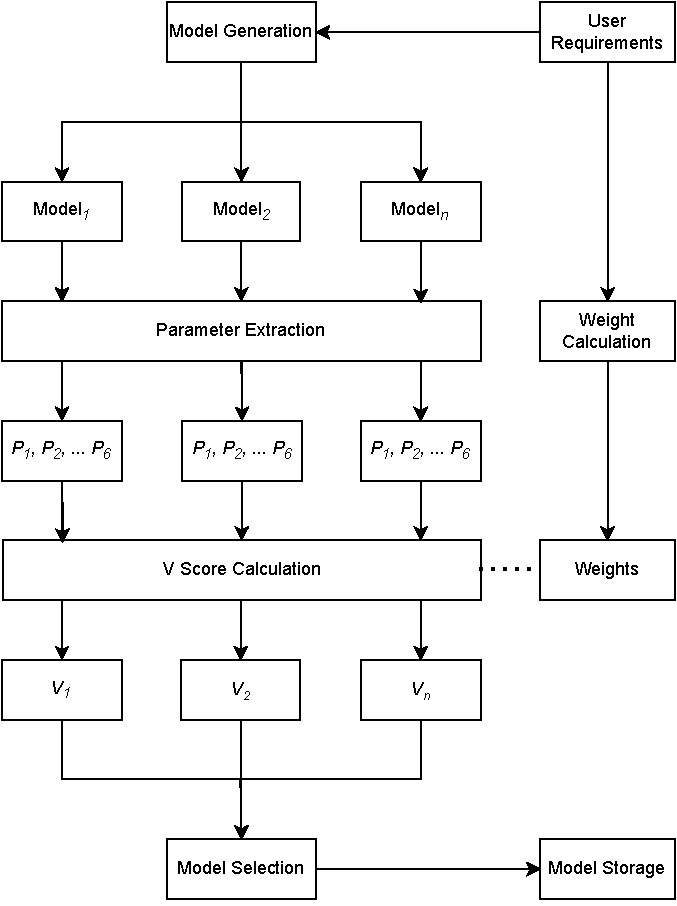
\includegraphics[width=1.4\columnwidth]{math_model_relaxed.pdf}
    \caption{Model Selection Approach}
    \label{fig:model_selection_approach}
\end{figure*}

% Best model Performance chart
\begin{figure*}[H]
    \begin{subfigure}{\columnwidth}
        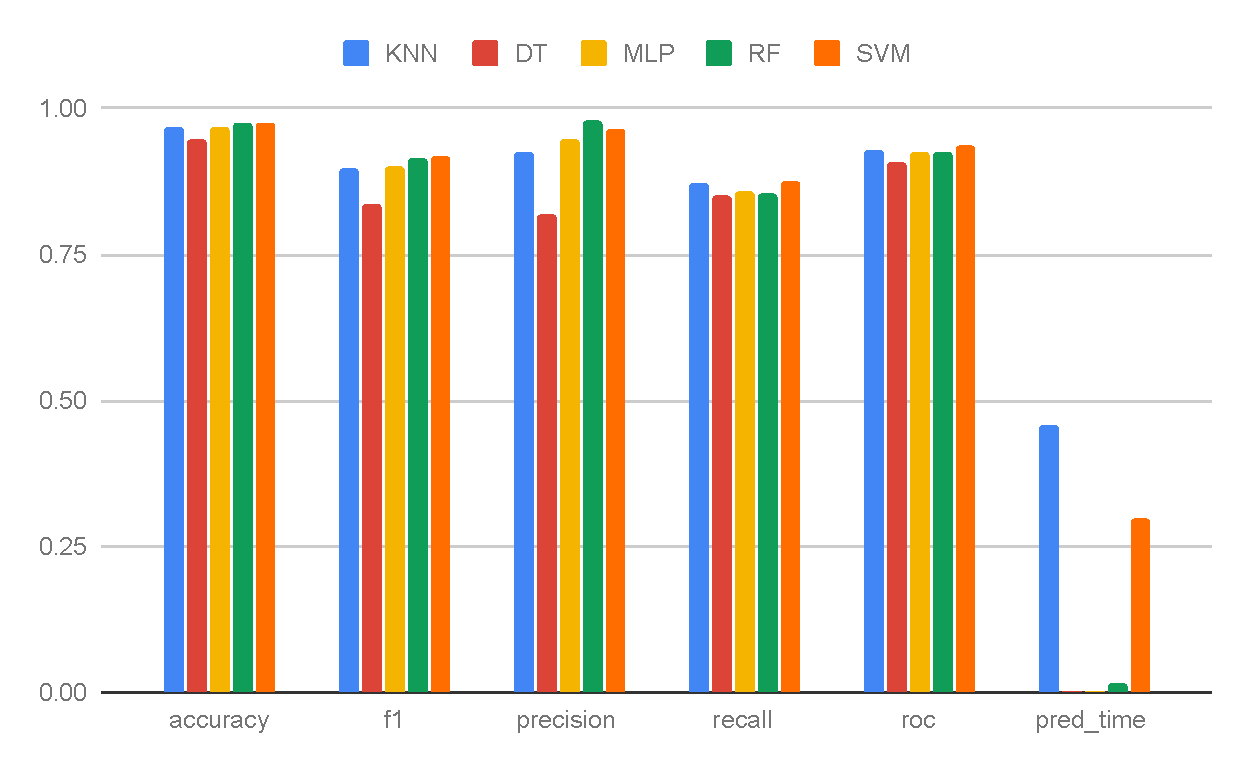
\includegraphics[width=0.9\columnwidth]{perf_ds_1.pdf}
        \caption{Dataset 1}\label{fig:performance_results_dataset_1}
    \end{subfigure}
    \begin{subfigure}{\columnwidth}
        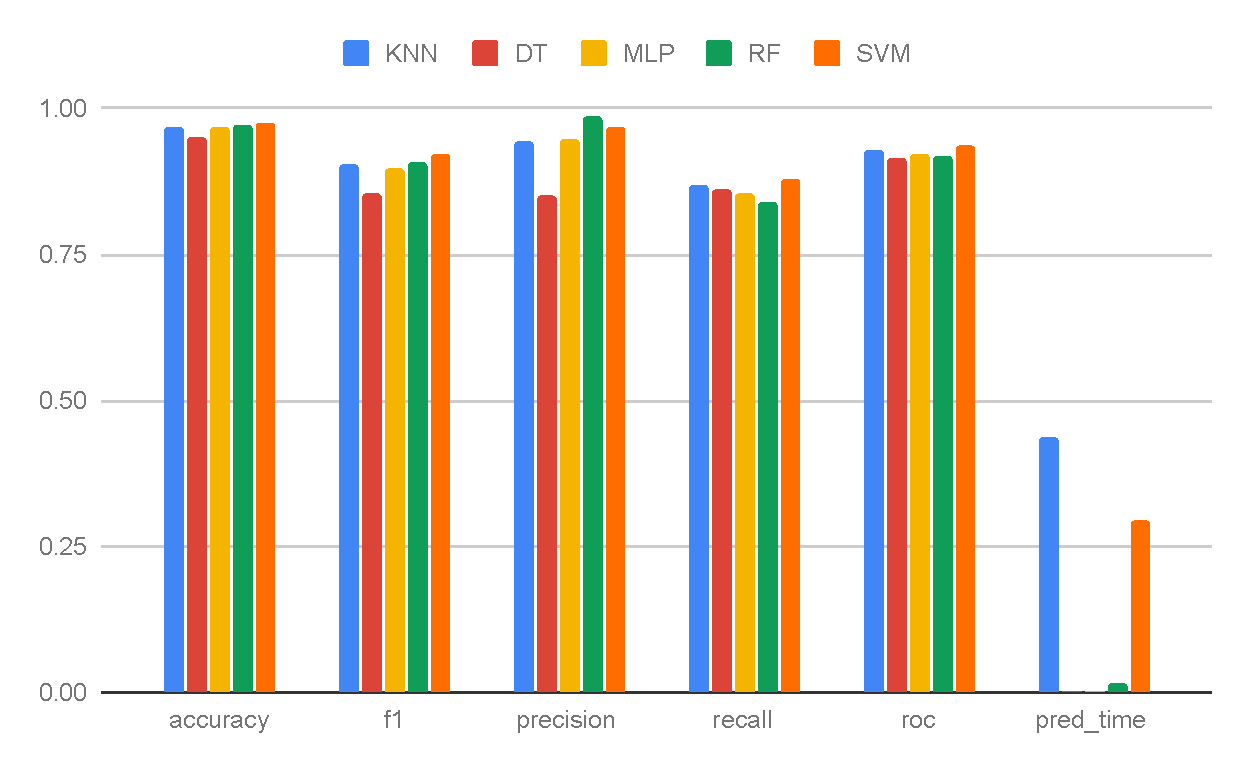
\includegraphics[width=0.9\columnwidth]{perf_ds_2.pdf}
        \caption{Dataset 2}\label{fig:performance_results_dataset_2}
    \end{subfigure}
    \begin{subfigure}{\columnwidth}
        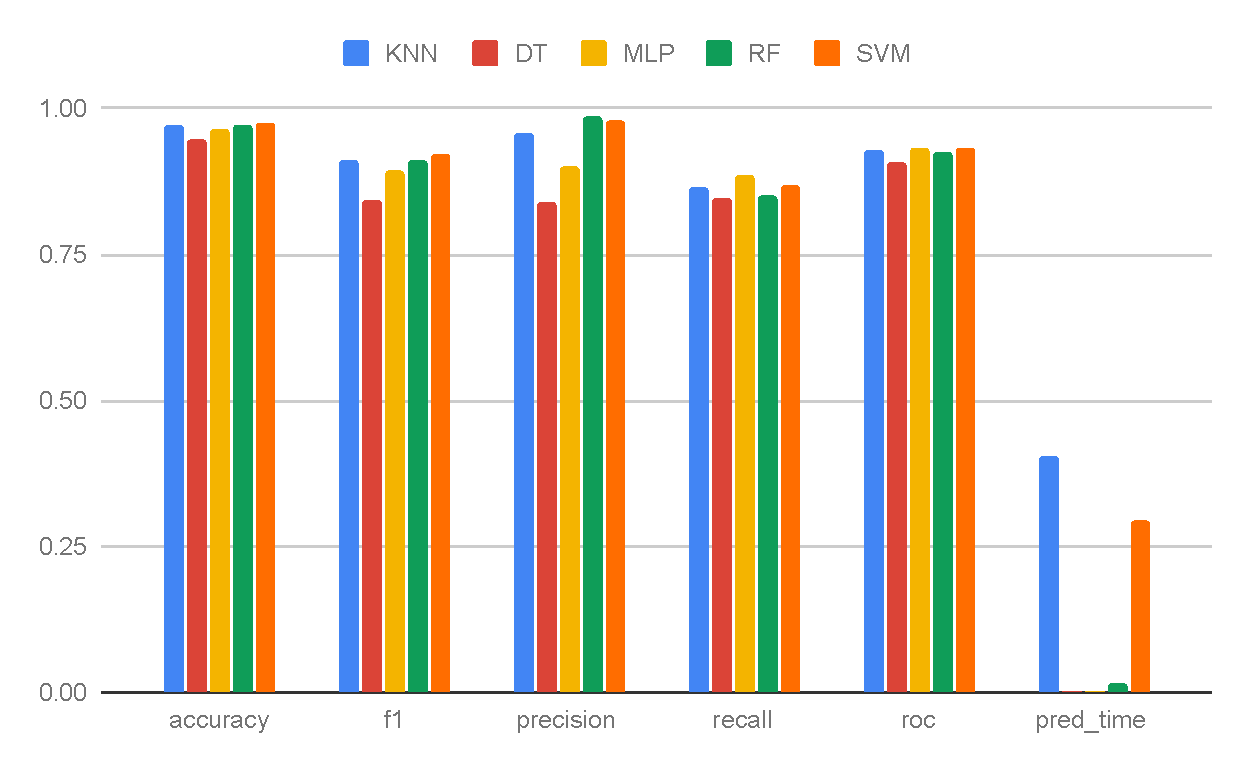
\includegraphics[width=0.9\columnwidth]{perf_ds_3.pdf}
        \caption{Dataset 3}\label{fig:performance_results_dataset_3}
    \end{subfigure}
    \begin{subfigure}{\columnwidth}
        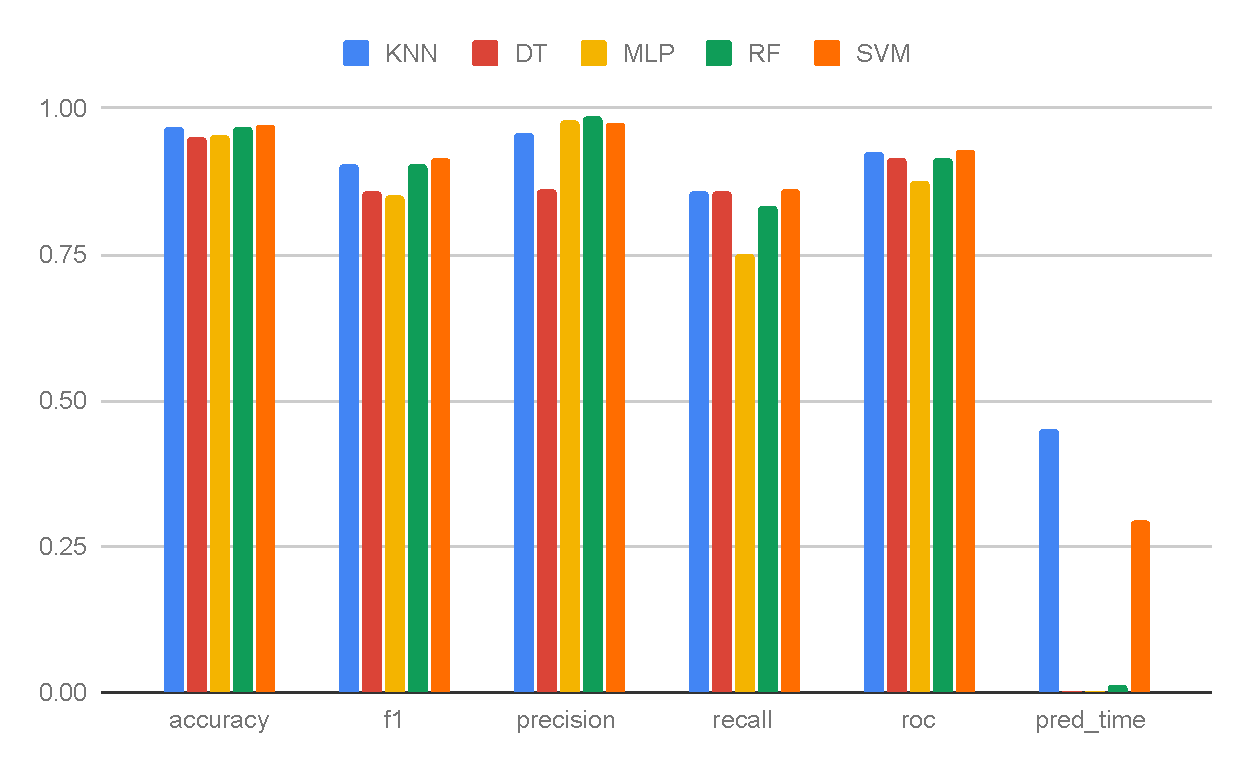
\includegraphics[width=0.9\columnwidth]{perf_ds_4.pdf}
        \caption{Dataset 4}\label{fig:performance_results_dataset_4}
    \end{subfigure}
    \caption{Perfromance Results}\label{fig:performance_results}
\end{figure*}

\begin{figure*}[H]
    \raggedright
    \begin{subfigure}{\columnwidth}
        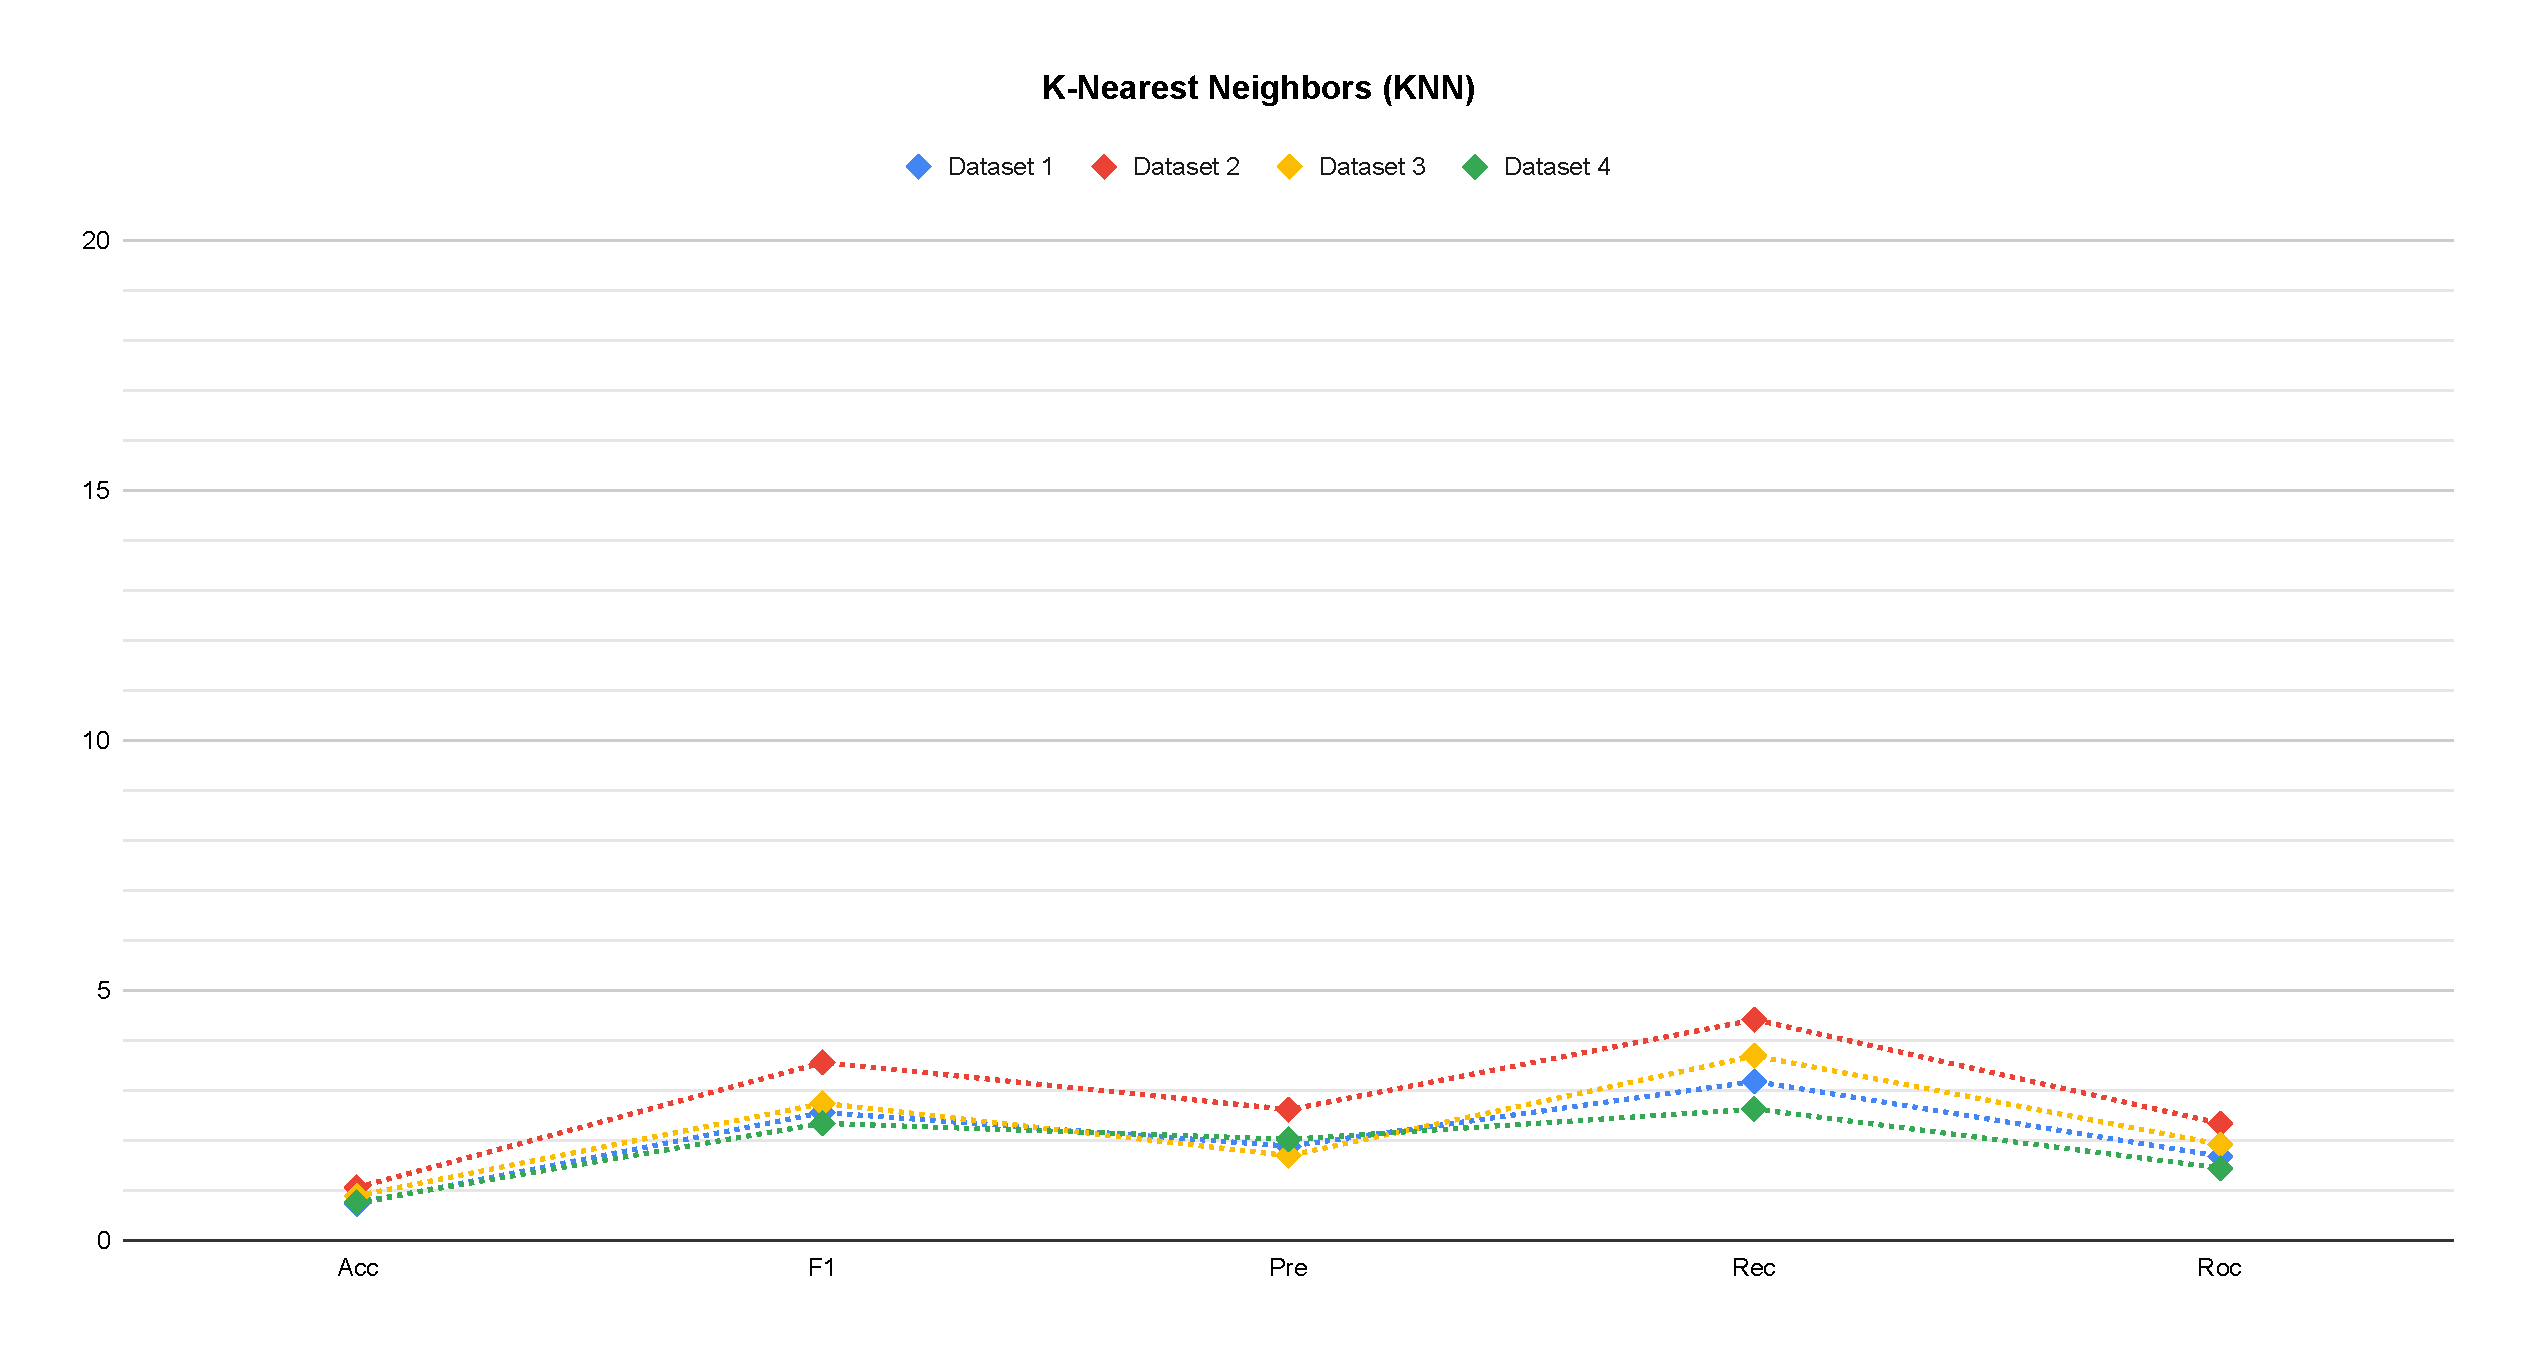
\includegraphics[width=0.9\columnwidth]{delta_KNN.pdf}
        \captionb{K-Nearest Neighbors Model}\label{fig:performance_delta_knn}
    \end{subfigure}
    \begin{subfigure}{\columnwidth}
        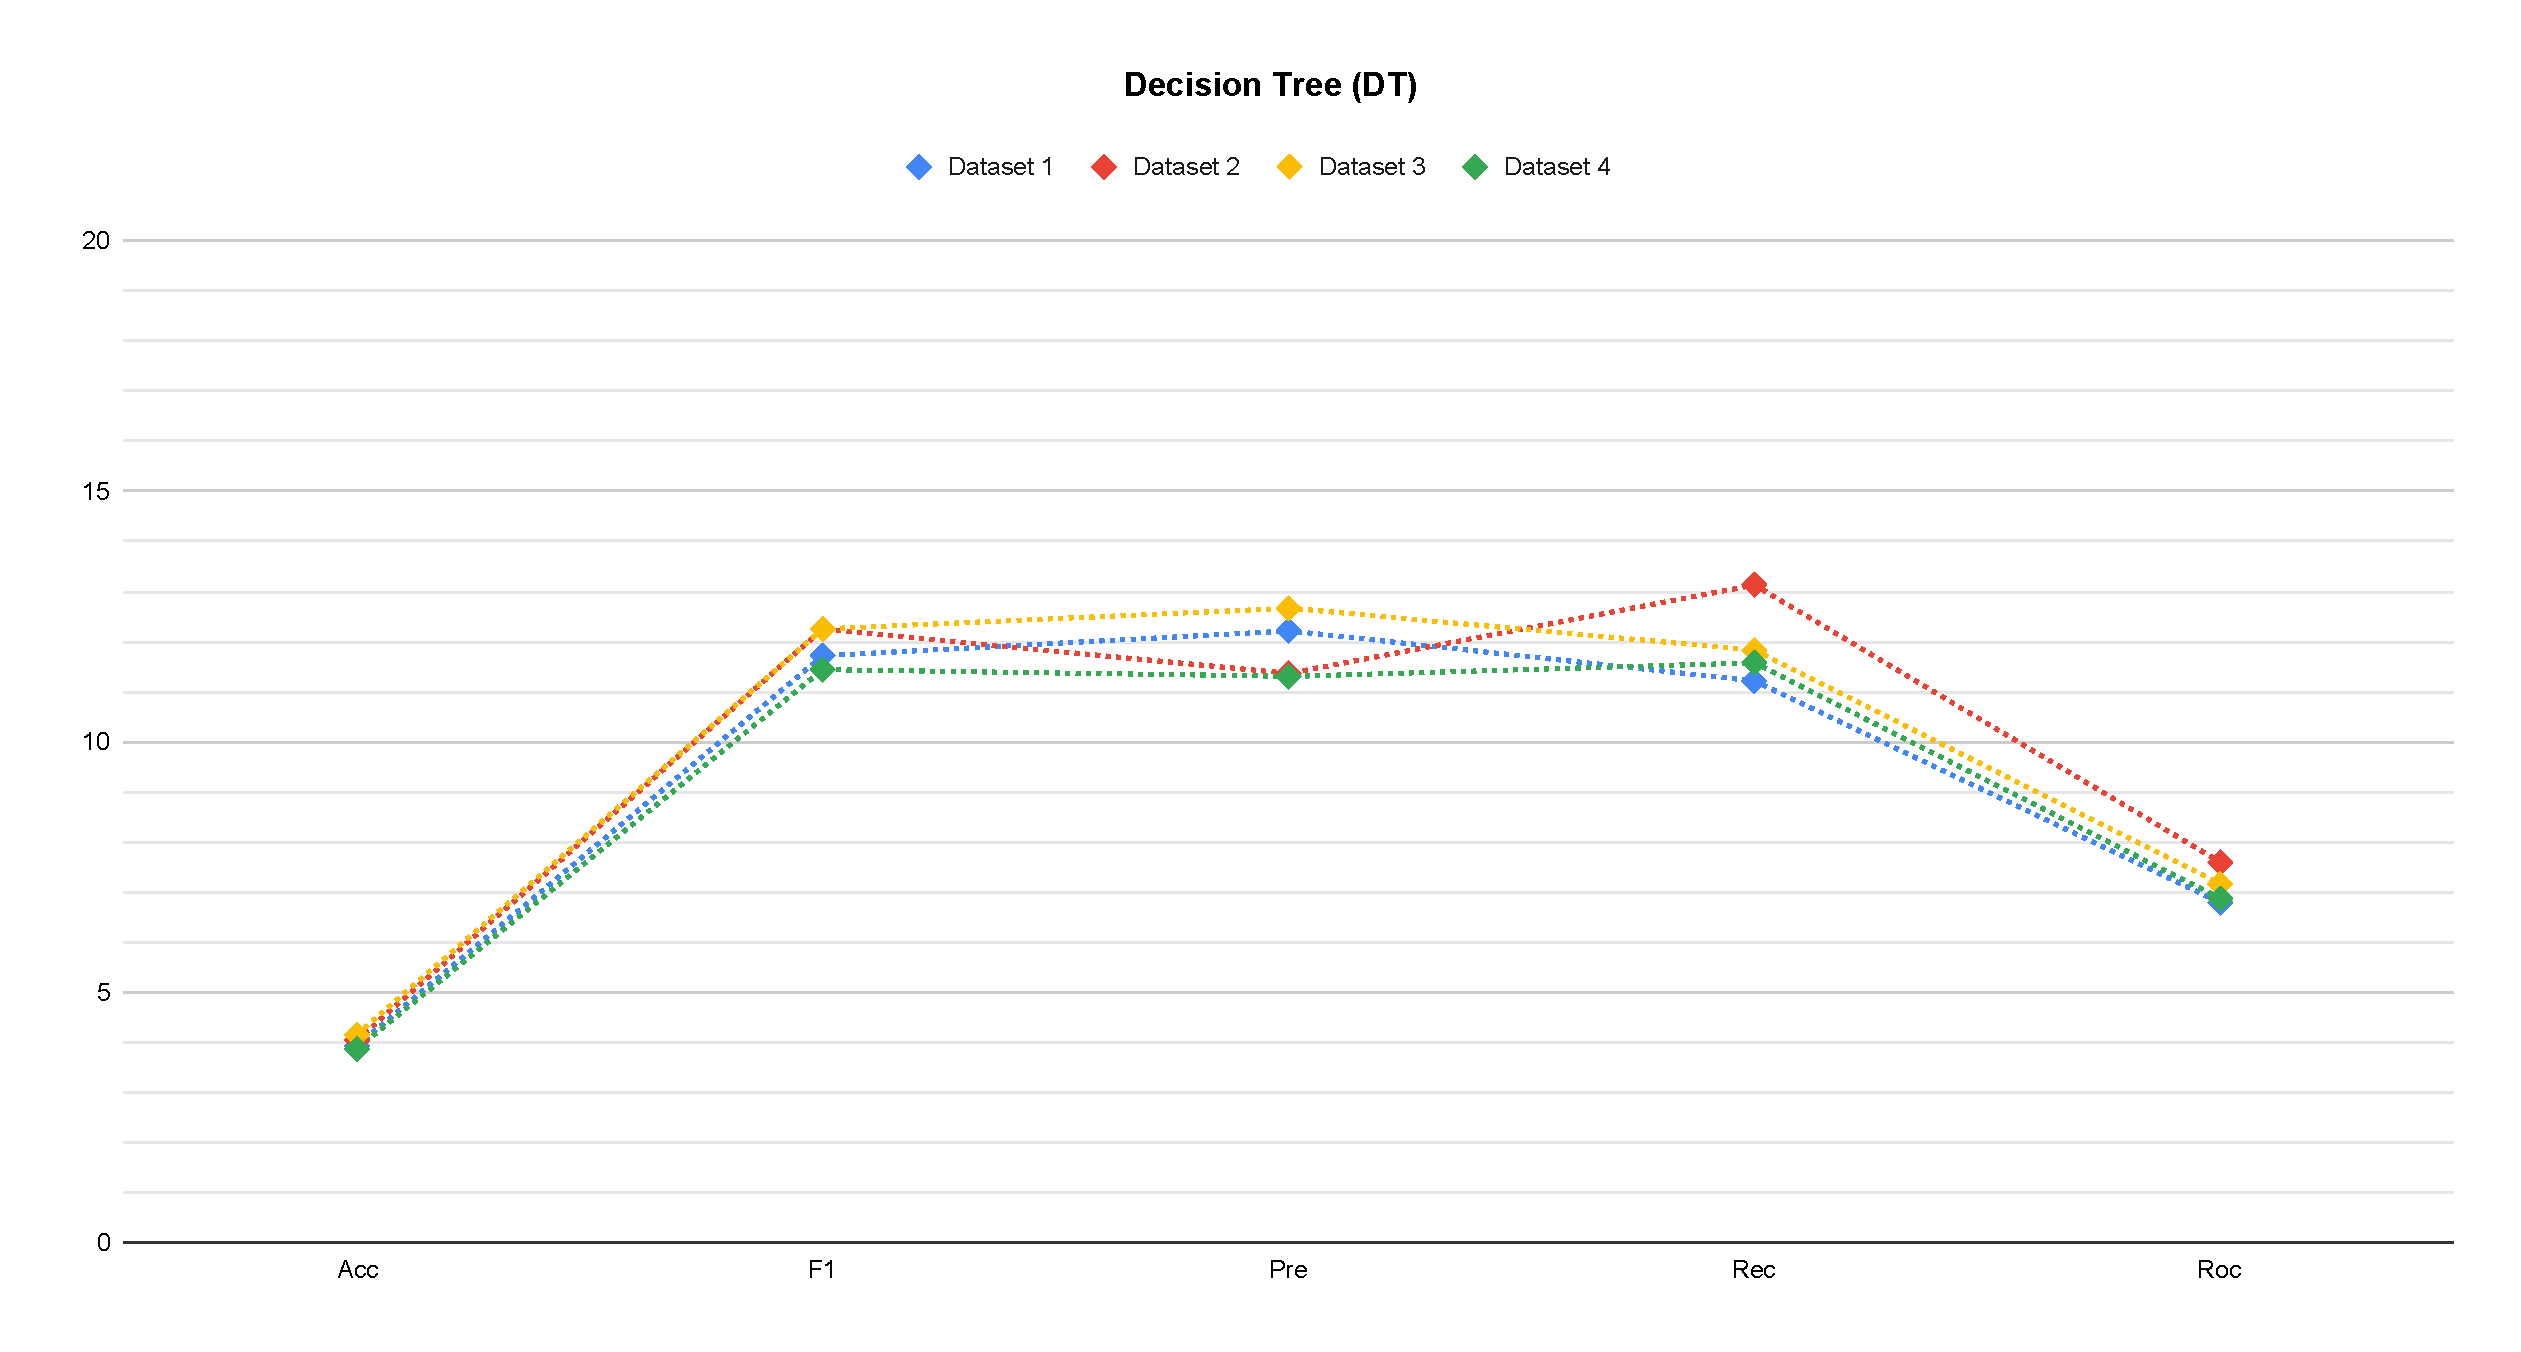
\includegraphics[width=0.9\columnwidth]{delta_DT.pdf}
        \captionb{Decision Tree Model}\label{fig:performance_delta_dt}
    \end{subfigure}
    \begin{subfigure}{\columnwidth}
        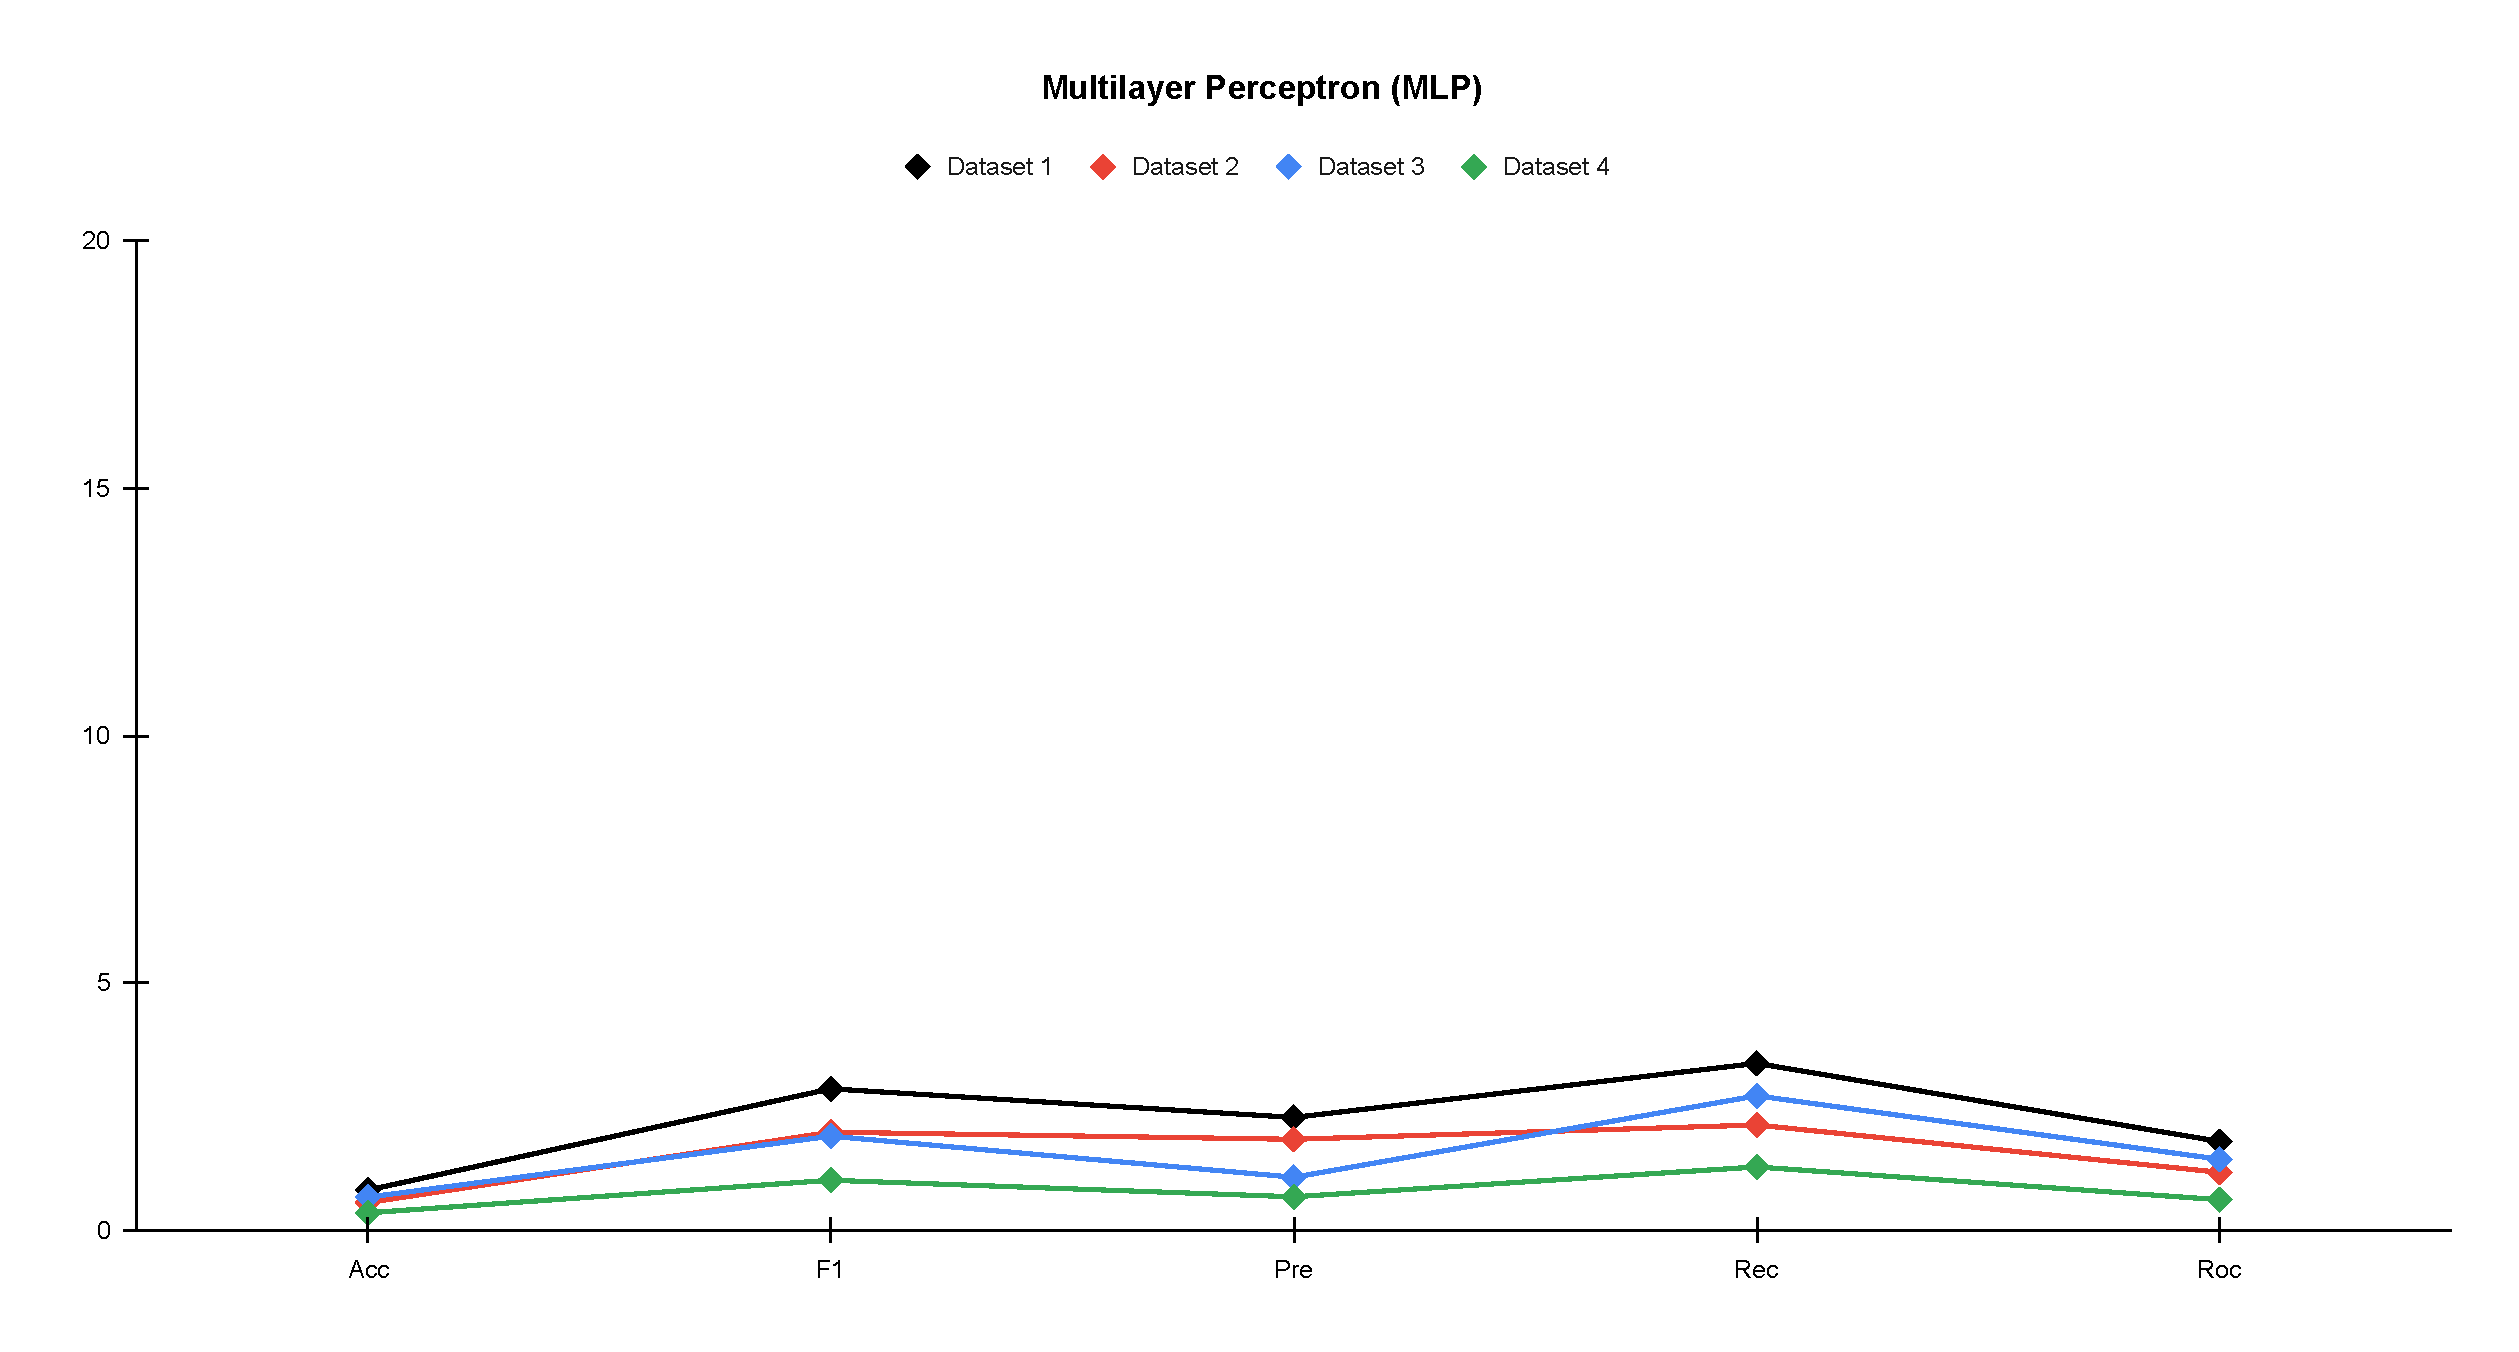
\includegraphics[width=0.9\columnwidth]{delta_MLP.pdf}
        \captionb{Multilayer Perceptron Model}\label{fig:performance_delta_mlp}
    \end{subfigure}
    \begin{subfigure}{\columnwidth}
        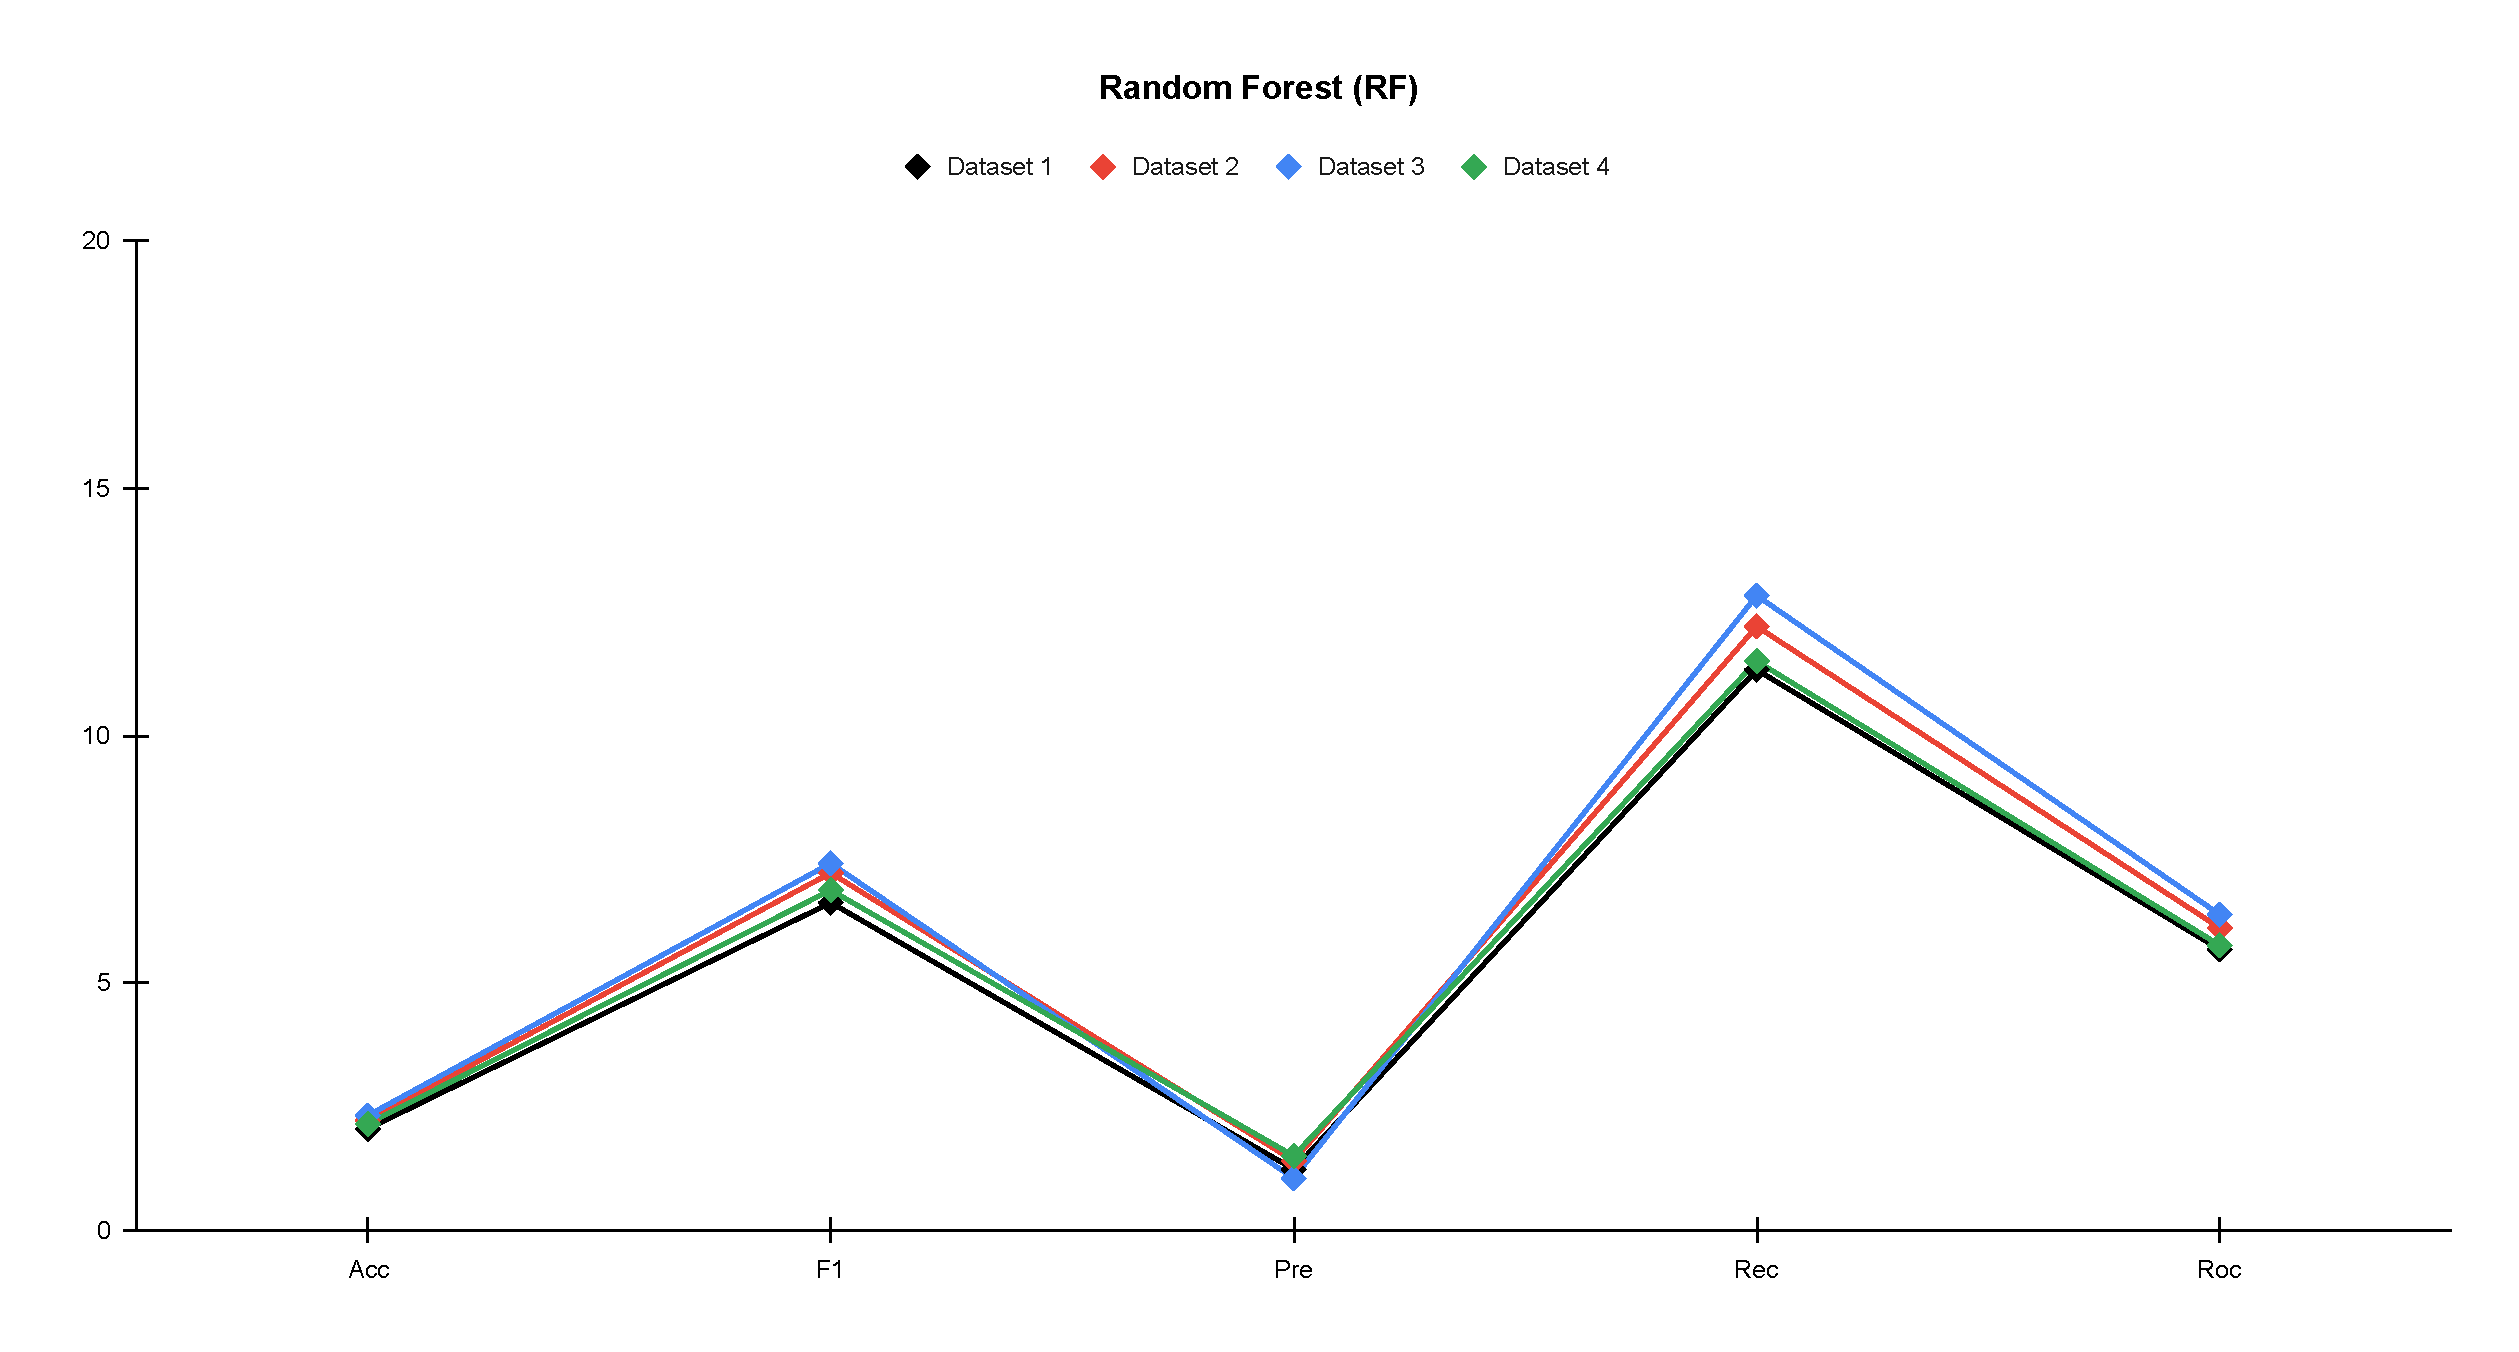
\includegraphics[width=0.9\columnwidth]{delta_RF.pdf}
        \captionb{Random Forest Model}\label{fig:performance_delta_rf}
    \end{subfigure}
    \begin{subfigure}{\columnwidth}
        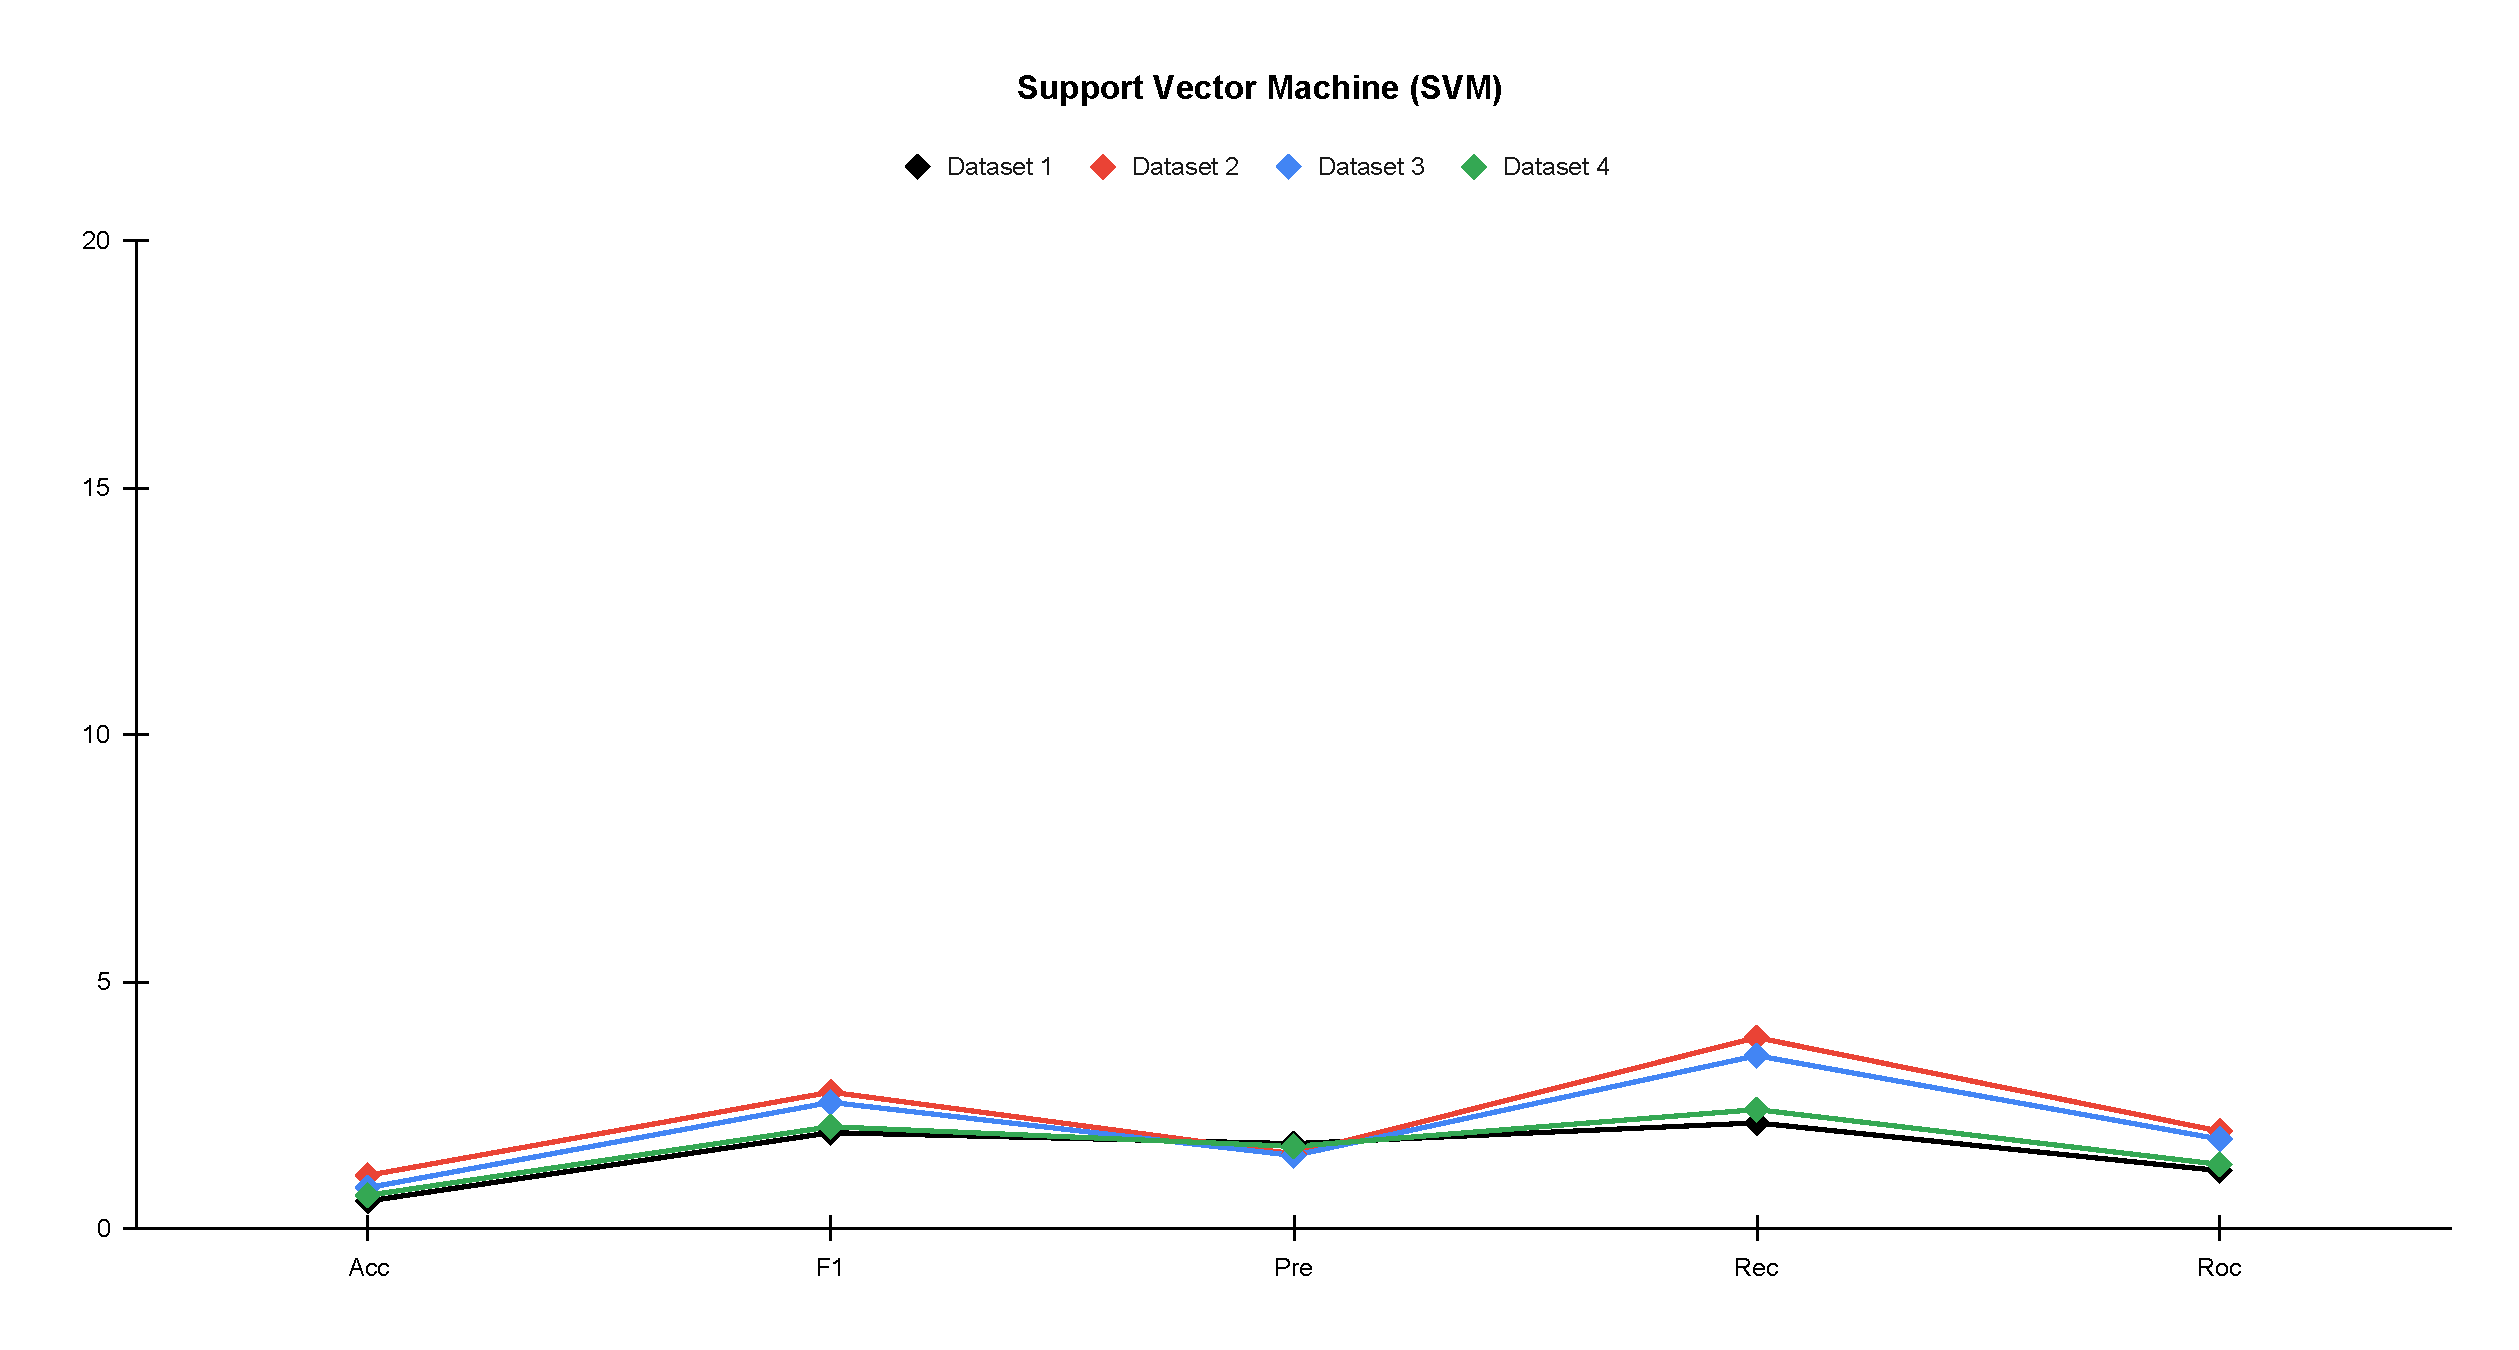
\includegraphics[width=0.9\columnwidth]{delta_SVM.pdf}
        \captionb{Support Vector Machine Model}\label{fig:performance_delta_svm}
    \end{subfigure}
    \captionb{Average performance error of the models}\label{fig:average_error}
\end{figure*}

\clearpage
\begin{table}[H]
    \caption{Vscores of Models}\label{tab:vscores_models}
    \begin{tabular*}{\tblwidth}{@{}FKKKK@{}}
        \toprule
        \bfrow Models & Dataset 1 & Dataset 2 & Dataset 3 & Dataset 4 \\
        \midrule
        KNN & 2.747 & 2.758 & 2.774 & 2.760 \\
        DT & 2.643 & 2.684 & 2.658 & 2.687 \\
        MLP & 2.782 & 2.771 & 2.766 & 2.674 \\
        RF & \textbf{2.807} & 2.795 & 2.803 & 2.786 \\
        SVM & 2.482 & \textbf{2.808} & \textbf{2.803} & \textbf{2.790} \\
        \bottomrule
    \end{tabular*}
\end{table}

% Best model Performance tabular
\begin{table}[hbt]
    \caption{Performance of models trained on dataset 1} \label{tab:performance_of_models_trained_on_dataset_1}
    \begin{tabular*}{\tblwidth}{@{}FKKKHK@{}}
        \toprule
        \bfrow Metric & KNN$_1$ & DT$_1$ & MLP$_1$ & RF$_1$ & SVM$_1$ \\
        \midrule
        Accuracy & 96.72 & 94.46 & 96.89 & 97.33 & 97.40 \\
        F1 & 89.71 & 83.43 & 90.05 & 91.30 & 91.69 \\
        Precision & 92.53 & 81.86 &94.71 &  97.95 & 96.43 \\
        Recall & 87.06 & 85.06 & 85.84 & 85.50 & 87.40 \\
        ROC & 92.84 & 90.68 & 92.45 & 92.57 & 93.38 \\
        Time(s) & 0.457 & 0.001 & 0.002 & 0.015 & 0.297 \\
        V$_{score}$ & 2.747 & 2.643 & 2.782 & 2.807 & 2.482 \\
        \bottomrule
    \end{tabular*}
\end{table}

\begin{table}[hbt]
    \caption{Performance of models trained on dataset 2} \label{tab:performance_of_models_trained_on_dataset_2}
    \begin{tabular*}{\tblwidth}{@{}FKKKKH@{}}
        \toprule
        \bfrow Metric & KNN$_2$ & DT$_2$ & MLP$_2$ & RF$_2$ & SVM$_2$ \\
        \midrule
        Accuracy & 96.83 & 95.04 & 96.69 & 97.09 & 97.46 \\
        F1 & 90.28 & 85.50 & 89.73 & 90.75 & 92.15 \\
        Precision & 94.25 & 84.90 & 94.73 & 98.60 & 96.79 \\
        Recall & 86.63 & 86.09 & 85.23 & 84.05 & 87.93 \\
        ROC & 92.77 & 91.48 & 92.13 & 91.90 & 93.66 \\
        Time(s) & 0.435 & 0.001 & 0.003 & 0.014 & 0.295 \\
        V$_{score}$ & 2.758 & 2.684 & 2.772 & 2.795 & 2.808 \\
        \bottomrule
    \end{tabular*}
\end{table}

\begin{table}[hbt]
    \caption{Performance of models trained on dataset 3} \label{tab:performance_of_models_trained_on_dataset_3}
    \begin{tabular*}{\tblwidth}{@{}FKKKKH@{}}
        \toprule
        \bfrow Metric & KNN$_3$ & DT$_3$ & MLP$_3$ & RF$_3$ & SVM$_3$ \\
        \midrule
        Accuracy & 97.07 & 94.64 & 96.41 & 97.22 & 97.44 \\
        F1 & 90.93 & 84.30 & 89.34 & 91.21 & 92.00 \\
        Precision & 95.82 & 83.81 & 90.13 & 98.37 & 97.81 \\
        Recall & 86.53 & 84.80 & 88.57 & 85.02 & 86.85 \\
        ROC & 92.87 & 90.73 & 93.29 & 92.36 & 93.22 \\
        Time(s) & 0.404 & 0.001 & 0.002 & 0.017 & 0.293 \\
        V$_{score}$ & 2.774 & 2.658 & 2.766 & 2.803 & 2.803 \\
        \bottomrule
    \end{tabular*}
\end{table}

\begin{table}[hbt]
    \caption{Performance of models trained on dataset 4} \label{tab:performance_of_models_trained_on_dataset_4}
    \begin{tabular*}{\tblwidth}{@{}FKKKKH@{}}
        \toprule
        \bfrow Metric & KNN$_4$ & DT$_4$ & MLP$_4$ & RF$_4$ & SVM$_4$ \\
        \midrule
        Accuracy & 96.84 & 94.99 & 95.34 & 96.88 & 97.15 \\
        F1 & 90.52 & 85.73 & 85.01 & 90.37 & 91.39 \\
        Precision & 95.71 & 85.91 & 97.83 & 98.65 & 97.41 \\
        Recall & 85.86 & 85.55 & 75.15 & 83.37 & 86.07 \\
        ROC & 92.52 & 91.28 & 87.40 & 91.56 & 92.79 \\
        Time(s) & 0.452 & 0.001 & 0.002 & 0.014 & 0.294 \\
        V$_{score}$ & 2.760 & 2.687 & 2.674 & 2.786 & 2.790 \\
        \bottomrule
    \end{tabular*}
\end{table}


\begin{table}[H]
    \caption{Performance of K Nearest Neighbors Models calculated on}\label{tab:performance_of_k_nearest_neighbors_models_multi}
    \begin{subtable}{\tblwidth}
        \caption{Dataset 1 and Dataset 2}
        \begin{tabular*}{\tblwidth}{@{}F|KKKK|KKKK@{}}
            \toprule
            \bfrow\multirow{2}{*}{Metric} & \multicolumn{4}{K|}{Dataset 1} & \multicolumn{4}{K}{Dataset 2} \\
            \bfrow & KNN$_1$ & KNN$_2$ & KNN$_3$ & KNN$_4$ & KNN$_1$ & KNN$_2$ & KNN$_3$ & KNN$_4$ \\
            \midrule
            Accuracy
            & 0.97 & 0.96 & 0.96 & 0.96 & 0.97 & 0.97 & 0.96 & 0.96 \\
            F1
            & 0.93 & 0.90 & 0.90 & 0.90 & 0.91 & 0.93 & 0.90 & 0.90 \\
            Precision
            & 0.96 & 0.94 & 0.95 & 0.94 & 0.95 & 0.96 & 0.95 & 0.95 \\
            Recall
            & 0.90 & 0.86 & 0.86 & 0.86 & 0.87 & 0.90 & 0.86 & 0.86 \\
            ROC
            & 0.94 & 0.92 & 0.92 & 0.92 & 0.93 & 0.94 & 0.92 & 0.92 \\
            \bottomrule
        \end{tabular*}
    \end{subtable}
\end{table}

\begin{table}[H]
    \ContinuedFloat
    \begin{subtable}{\tblwidth}
        \caption{Dataset 3 and Dataset 4}
        \begin{tabular*}{\tblwidth}{@{}F|KKKK|KKKK@{}}
            \toprule
            \bfrow\multirow{2}{*}{Metric} & \multicolumn{4}{K|}{Dataset 3} & \multicolumn{4}{K}{Dataset 4} \\
            \bfrow & KNN$_1$ & KNN$_2$ & KNN$_3$ & KNN$_4$ & KNN$_1$ & KNN$_2$ & KNN$_3$ & KNN$_4$ \\
            \midrule
            Accuracy
            & 0.97 & 0.96 & 0.97 & 0.96 & 0.96 & 0.96 & 0.96 & 0.97 \\
            F1
            & 0.90 & 0.90 & 0.93 & 0.90 & 0.90 & 0.89 & 0.90 & 0.92 \\
            Precision
            & 0.94 & 0.94 & 0.96 & 0.94 & 0.94 & 0.94 & 0.94 & 0.96 \\
            Recall
            & 0.87 & 0.86 & 0.89 & 0.87 & 0.87 & 0.85 & 0.86 & 0.89 \\
            ROC
            & 0.93 & 0.92 & 0.94 & 0.93 & 0.93 & 0.92 & 0.92 & 0.94 \\
            \bottomrule
        \end{tabular*}
    \end{subtable}
\end{table}


\begin{table}[H]
    \caption{Performance of Decision Tree Model calculated on}\label{tab:performance_decision_tree_multi}
    \begin{subtable}{\tblwidth}
        \caption{Dataset 1 and Dataset 2}
        \begin{tabular*}{\tblwidth}{@{}F|KKKK|KKKK@{}}
            \toprule
            \bfrow\multirow{2}{*}{Metric} & \multicolumn{4}{K|}{Dataset 1} & \multicolumn{4}{K}{Dataset 2} \\
            \bfrow & DT$_1$ & DT$_2$ & DT$_3$ & DT$_4$ & DT$_1$ & DT$_2$ & DT$_3$ & DT$_4$ \\
            \midrule
            Accuracy
            & 0.98 & 0.94 & 0.94 & 0.94 & 0.94 & 0.98 & 0.94 & 0.94 \\
            F1
            & 0.98 & 0.94 & 0.94 & 0.94 & 0.94 & 0.98 & 0.94 & 0.94 \\
            Precision
            & 0.95 & 0.85 & 0.84 & 0.85 & 0.83 & 0.96 & 0.83 & 0.85 \\
            Recall
            & 0.96 & 0.82 & 0.84 & 0.85 & 0.86 & 0.96 & 0.85 & 0.84 \\
            ROC
            & 0.97 & 0.89 & 0.90 & 0.91 & 0.91 & 0.97 & 0.90 & 0.90 \\
            \bottomrule
        \end{tabular*}
    \end{subtable}
\end{table}

\begin{table}[H]
    \begin{subtable}{\tblwidth}
        \caption{Dataset 3 and Dataset 4}
        \begin{tabular*}{\tblwidth}{@{}F|KKKK|KKKK@{}}
            \toprule
            \bfrow\multirow{2}{*}{Metric} & \multicolumn{4}{K|}{Dataset 3} & \multicolumn{4}{K}{Dataset 4} \\
            \bfrow & DT$_1$ & DT$_2$ & DT$_3$ & DT$_4$ & DT$_1$ & DT$_2$ & DT$_3$ & DT$_4$ \\
            \midrule
            Accuracy
            & 0.94 & 0.94 & 0.98 & 0.95 & 0.94 & 0.94 & 0.94 & 0.98 \\
            F1
            & 0.94 & 0.94 & 0.98 & 0.95 & 0.94 & 0.94 & 0.94 & 0.98 \\
            Precision
            & 0.84 & 0.85 & 0.95 & 0.85 & 0.83 & 0.85 & 0.83 & 0.96 \\
            Recall
            & 0.85 & 0.84 & 0.96 & 0.85 & 0.85 & 0.84 & 0.84 & 0.96 \\
            ROC
            & 0.91 & 0.90 & 0.97 & 0.91 & 0.90 & 0.90 & 0.90 & 0.97 \\
            \bottomrule
        \end{tabular*}
    \end{subtable}
\end{table}


\begin{table}[H]
    \caption{Performance of Multilayer Perceptron Models calculated on}\label{tab:performance_multilayer_perceptron_multi}
    \begin{subtable}{\tblwidth}
        \caption{Dataset 1 and Dataset 2}
        \begin{tabular*}{\tblwidth}{@{}F|KKKK|KKKK@{}}
            \toprule
            \bfrow\multirow{2}{*}{Metric} & \multicolumn{4}{K|}{Dataset 1} & \multicolumn{4}{K}{Dataset 2} \\
            \bfrow & MLP$_1$ & MLP$_2$ & MLP$_3$ & MLP$_4$ & MLP$_1$ & MLP$_2$ & MLP$_3$ & MLP$_4$ \\
            \midrule
            Accuracy
            & 0.97 & 0.96 & 0.96 & 0.95 & 0.96 & 0.97 & 0.96 & 0.95 \\
            F1
            & 0.92 & 0.90 & 0.89 & 0.85 & 0.89 & 0.91 & 0.89 & 0.85 \\
            Precision
            & 0.97 & 0.95 & 0.89 & 0.97 & 0.95 & 0.97 & 0.89 & 0.97 \\
            Recall
            & 0.88 & 0.85 & 0.88 & 0.75 & 0.85 & 0.87 & 0.88 & 0.75 \\
            ROC
            & 0.93 & 0.92 & 0.93 & 0.87 & 0.92 & 0.93 & 0.93 & 0.87 \\
            \bottomrule
        \end{tabular*}
    \end{subtable}
\end{table}

\begin{table}[H]
    \begin{subtable}{\tblwidth}
        \caption{Dataset 3 and Dataset 4}
        \begin{tabular*}{\tblwidth}{@{}F|KKKK|KKKK@{}}
            \toprule
            \bfrow\multirow{2}{*}{Metric} & \multicolumn{4}{K|}{Dataset 3} & \multicolumn{4}{K}{Dataset 4} \\
            \bfrow & MLP$_1$ & MLP$_2$ & MLP$_3$ & MLP$_4$ & MLP$_1$ & MLP$_2$ & MLP$_3$ & MLP$_4$ \\
            \midrule
            Accuracy
            & 0.96 & 0.96 & 0.96 & 0.95 & 0.96 & 0.96 & 0.96 & 0.95 \\
            F1
            & 0.89 & 0.90 & 0.90 & 0.85 & 0.89 & 0.90 & 0.88 & 0.86 \\
            Precision
            & 0.94 & 0.94 & 0.90 & 0.97 & 0.95 & 0.95 & 0.89 & 0.98 \\
            Recall
            & 0.85 & 0.85 & 0.91 & 0.75 & 0.85 & 0.85 & 0.88 & 0.76 \\
            ROC
            & 0.92 & 0.92 & 0.94 & 0.87 & 0.92 & 0.92 & 0.93 & 0.88 \\
            \bottomrule
        \end{tabular*}
    \end{subtable}
\end{table}


\begin{table}[H]
    \caption{Performance of Random Forest Models calculated on}\label{tab:performance_random_forest_multi}
    \begin{subtable}{\tblwidth}
        \caption{Dataset 1 and Dataset 2}
        \begin{tabular*}{\tblwidth}{@{}F|KKKK|KKKK@{}}
            \toprule
            \bfrow\multirow{2}{*}{Metric} & \multicolumn{4}{K|}{Dataset 1} & \multicolumn{4}{K}{Dataset 2} \\
            \bfrow & RF$_1$ & RF$_2$ & RF$_3$ & RF$_4$ & RF$_1$ & RF$_2$ & RF$_3$ & RF$_4$ \\
            \midrule
            Accuracy
            & 0.99 & 0.96 & 0.96 & 0.96 & 0.97 & 0.99 & 0.97 & 0.97 \\
            F1
            & 0.98 & 0.90 & 0.90 & 0.90 & 0.91 & 0.97 & 0.90 & 0.91 \\
            Precision
            & 0.99 & 0.98 & 0.98 & 0.98 & 0.98 & 0.99 & 0.98 & 0.98 \\
            Recall
            & 0.96 & 0.83 & 0.83 & 0.84 & 0.85 & 0.96 & 0.84 & 0.84 \\
            ROC
            & 0.98 & 0.91 & 0.91 & 0.91 & 0.92 & 0.98 & 0.91 & 0.92 \\
            \bottomrule
        \end{tabular*}
    \end{subtable}
\end{table}

\begin{table}[H]
    \begin{subtable}{\tblwidth}
        \caption{Dataset 3 and Dataset 4}
        \begin{tabular*}{\tblwidth}{@{}F|KKKK|KKKK@{}}
            \toprule
            \bfrow\multirow{2}{*}{Metric} & \multicolumn{4}{K|}{Dataset 3} & \multicolumn{4}{K}{Dataset 4} \\
            \bfrow & RF$_1$ & RF$_2$ & RF$_3$ & RF$_4$ & RF$_1$ & RF$_2$ & RF$_3$ & RF$_4$ \\
            \midrule
            Accuracy
            & 0.97 & 0.97 & 0.99 & 0.97 & 0.97 & 0.97 & 0.97 & 0.99 \\
            F1
            & 0.91 & 0.91 & 0.97 & 0.90 & 0.91 & 0.90 & 0.90 & 0.97 \\
            Precision
            & 0.97 & 0.97 & 0.99 & 0.97 & 0.98 & 0.98 & 0.98 & 0.99 \\
            Recall
            & 0.85 & 0.85 & 0.96 & 0.85 & 0.85 & 0.84 & 0.83 & 0.95 \\
            ROC
            & 0.92 & 0.92 & 0.98 & 0.92 & 0.92 & 0.91 & 0.91 & 0.97 \\
            \bottomrule
        \end{tabular*}
    \end{subtable}
\end{table}

\begin{table}[H]
    \caption{Performance of Support Vector Machine Models calculated on}\label{tab:performance_support_vector_machine_multi}
    \begin{subtable}{\tblwidth}
        \caption{Dataset 1 and Dataset 2}
        \begin{tabular*}{\tblwidth}{@{}F|KKKK|KKKK@{}}
            \toprule
            \bfrow\multirow{2}{*}{Metric} & \multicolumn{4}{K|}{Dataset 1} & \multicolumn{4}{K}{Dataset 2} \\
            \bfrow & SVM$_1$ & SVM$_2$ & SVM$_3$ & SVM$_4$ & SVM$_1$ & SVM$_2$ & SVM$_3$ & SVM$_4$ \\
            \midrule
            Accuracy
            & 0.97 & 0.97 & 0.97 & 0.97 & 0.97 & 0.98 & 0.97 & 0.97 \\
            F1
            & 0.93 & 0.91 & 0.91 & 0.91 & 0.92 & 0.94 & 0.92 & 0.91 \\
            Precision
            & 0.98 & 0.97 & 0.97 & 0.97 & 0.97 & 0.98 & 0.97 & 0.96 \\
            Recall
            & 0.89 & 0.86 & 0.85 & 0.85 & 0.87 & 0.89 & 0.87 & 0.86 \\
            ROC
            & 0.94 & 0.92 & 0.92 & 0.92 & 0.93 & 0.94 & 0.93 & 0.93 \\
            \bottomrule
        \end{tabular*}
    \end{subtable}
\end{table}

\begin{table}[H]
    \begin{subtable}{\tblwidth}
        \caption{Dataset 3 and Dataset 4}
        \begin{tabular*}{\tblwidth}{@{}F|KKKK|KKKK@{}}
            \toprule
            \bfrow\multirow{2}{*}{Metric} & \multicolumn{4}{K|}{Dataset 3} & \multicolumn{4}{K}{Dataset 4} \\
            \bfrow & SVM$_1$ & SVM$_2$ & SVM$_3$ & SVM$_4$ & SVM$_1$ & SVM$_2$ & SVM$_3$ & SVM$_4$ \\
            \midrule
            Accuracy
            & 0.97 & 0.97 & 0.98 & 0.97 & 0.97 & 0.97 & 0.97 & 0.97 \\
            F1
            & 0.91 & 0.91 & 0.94 & 0.91 & 0.91 & 0.91 & 0.91 & 0.93 \\
            Precision
            & 0.96 & 0.96 & 0.98 & 0.96 & 0.96 & 0.96 & 0.97 & 0.98 \\
            Recall
            & 0.87 & 0.86 & 0.89 & 0.86 & 0.87 & 0.86 & 0.87 & 0.88 \\
            ROC
            & 0.93 & 0.93 & 0.94 & 0.93 & 0.93 & 0.92 & 0.93 & 0.94 \\
            \bottomrule
        \end{tabular*}
    \end{subtable}
\end{table}

\clearpage
\printcredits

\raggedright
\bibliographystyle{cas-model2-names}

\bibliography{cas-refs.bib}

\end{document}
